\documentclass[11pt,a4paper,]{article}
\usepackage[]{mathpazo}

\usepackage{amssymb,amsmath}
\usepackage{ifxetex,ifluatex}
\usepackage{fixltx2e} % provides \textsubscript
\ifnum 0\ifxetex 1\fi\ifluatex 1\fi=0 % if pdftex
  \usepackage[T1]{fontenc}
  \usepackage[utf8]{inputenc}
\else % if luatex or xelatex
  \usepackage{unicode-math}
  \defaultfontfeatures{Ligatures=TeX,Scale=MatchLowercase}
\fi
% use upquote if available, for straight quotes in verbatim environments
\IfFileExists{upquote.sty}{\usepackage{upquote}}{}
% use microtype if available
\IfFileExists{microtype.sty}{%
\usepackage[]{microtype}
\UseMicrotypeSet[protrusion]{basicmath} % disable protrusion for tt fonts
}{}
\PassOptionsToPackage{hyphens}{url} % url is loaded by hyperref
\usepackage[unicode=true]{hyperref}
\hypersetup{
            pdftitle={Meta-learning how to forecast time series},
            pdfkeywords={FFORMS (Feature-based FORecast-model Selection), Time series features, Random forest, Algorithm selection problem, Classsification},
            pdfborder={0 0 0},
            breaklinks=true}
\urlstyle{same}  % don't use monospace font for urls
\usepackage{geometry}
\geometry{left=2.5cm,right=2.5cm,top=2.5cm,bottom=2.5cm}
\usepackage[style=authoryear-comp,]{biblatex}
\addbibresource{FBF.bib}
\usepackage{longtable,booktabs}
% Fix footnotes in tables (requires footnote package)
\IfFileExists{footnote.sty}{\usepackage{footnote}\makesavenoteenv{long table}}{}
\IfFileExists{parskip.sty}{%
\usepackage{parskip}
}{% else
\setlength{\parindent}{0pt}
\setlength{\parskip}{6pt plus 2pt minus 1pt}
}
\setlength{\emergencystretch}{3em}  % prevent overfull lines
\providecommand{\tightlist}{%
  \setlength{\itemsep}{0pt}\setlength{\parskip}{0pt}}
\setcounter{secnumdepth}{5}

% set default figure placement to htbp
\makeatletter
\def\fps@figure{htbp}
\makeatother


\title{Meta-learning how to forecast time series}

%% MONASH STUFF

%% CAPTIONS
\RequirePackage{caption}
\DeclareCaptionStyle{italic}[justification=centering]
 {labelfont={bf},textfont={it},labelsep=colon}
\captionsetup[figure]{style=italic,format=hang,singlelinecheck=true}
\captionsetup[table]{style=italic,format=hang,singlelinecheck=true}

%% FONT
\RequirePackage{bera}
\RequirePackage{mathpazo}

%% HEADERS AND FOOTERS
\RequirePackage{fancyhdr}
\pagestyle{fancy}
\rfoot{\Large\sffamily\raisebox{-0.1cm}{\textbf{\thepage}}}
\makeatletter
\lhead{\textsf{\expandafter{\@title}}}
\makeatother
\rhead{}
\cfoot{}
\setlength{\headheight}{15pt}
\renewcommand{\headrulewidth}{0.4pt}
\renewcommand{\footrulewidth}{0.4pt}
\fancypagestyle{plain}{%
\fancyhf{} % clear all header and footer fields
\fancyfoot[C]{\sffamily\thepage} % except the center
\renewcommand{\headrulewidth}{0pt}
\renewcommand{\footrulewidth}{0pt}}

%% MATHS
\RequirePackage{bm,amsmath}
\allowdisplaybreaks

%% GRAPHICS
\RequirePackage{graphicx}
\setcounter{topnumber}{2}
\setcounter{bottomnumber}{2}
\setcounter{totalnumber}{4}
\renewcommand{\topfraction}{0.85}
\renewcommand{\bottomfraction}{0.85}
\renewcommand{\textfraction}{0.15}
\renewcommand{\floatpagefraction}{0.8}

%\RequirePackage[section]{placeins}

%% SECTION TITLES
\RequirePackage[compact,sf,bf]{titlesec}
\titleformat{\section}[block]
  {\fontsize{15}{17}\bfseries\sffamily}
  {\thesection}
  {0.4em}{}
\titleformat{\subsection}[block]
  {\fontsize{12}{14}\bfseries\sffamily}
  {\thesubsection}
  {0.4em}{}
\titlespacing{\section}{0pt}{*5}{*1}
\titlespacing{\subsection}{0pt}{*2}{*0.2}


%% TITLE PAGE
\def\Date{\number\day}
\def\Month{\ifcase\month\or
 January\or February\or March\or April\or May\or June\or
 July\or August\or September\or October\or November\or December\fi}
\def\Year{\number\year}

\makeatletter
\def\wp#1{\gdef\@wp{#1}}\def\@wp{??/??}
\def\jel#1{\gdef\@jel{#1}}\def\@jel{??}
\def\showjel{{\large\textsf{\textbf{JEL classification:}}~\@jel}}
\def\nojel{\def\showjel{}}
\def\addresses#1{\gdef\@addresses{#1}}\def\@addresses{??}
\def\cover{{\sffamily\setcounter{page}{0}
        \thispagestyle{empty}
        \placefig{2}{1.5}{width=5cm}{monash2}
        \placefig{16.9}{1.5}{width=2.1cm}{MBusSchool}
        \begin{textblock}{4}(16.9,4)ISSN 1440-771X\end{textblock}
        \begin{textblock}{7}(12.7,27.9)\hfill
        
\includegraphics[height=0.7cm]{AACSB}~~~
        
\includegraphics[height=0.7cm]{EQUIS}~~~
        
\includegraphics[height=0.7cm]{AMBA}
        \end{textblock}
        \vspace*{2cm}
        \begin{center}\Large
        Department of Econometrics and Business Statistics\\[.5cm]
        \footnotesize http://monash.edu/business/ebs/research/publications
        \end{center}\vspace{2cm}
        \begin{center}
        \fbox{\parbox{14cm}{\begin{onehalfspace}\centering\Huge\vspace*{0.3cm}
                \textsf{\textbf{\expandafter{\@title}}}\vspace{1cm}\par
                \LARGE\@author\end{onehalfspace}
        }}
        \end{center}
        \vfill
                \begin{center}\Large
                \Month~\Year\\[1cm]
                Working Paper \@wp
        \end{center}\vspace*{2cm}}}
\def\pageone{{\sffamily\setstretch{1}%
        \thispagestyle{empty}%
        \vbox to \textheight{%
        \raggedright\baselineskip=1.2cm
     {\fontsize{24.88}{30}\sffamily\textbf{\expandafter{\@title}}}
        \vspace{2cm}\par
        \hspace{1cm}\parbox{14cm}{\sffamily\large\@addresses}\vspace{1cm}\vfill
        \hspace{1cm}{\large\Date~\Month~\Year}\\[1cm]
        \hspace{1cm}\showjel\vss}}}
\def\blindtitle{{\sffamily
     \thispagestyle{plain}\raggedright\baselineskip=1.2cm
     {\fontsize{24.88}{30}\sffamily\textbf{\expandafter{\@title}}}\vspace{1cm}\par
        }}
\def\titlepage{{\cover\newpage\pageone\newpage\blindtitle}}

\def\blind{\def\titlepage{{\blindtitle}}\let\maketitle\blindtitle}
\def\titlepageonly{\def\titlepage{{\pageone\end{document}}}}
\def\nocover{\def\titlepage{{\pageone\newpage\blindtitle}}\let\maketitle\titlepage}
\let\maketitle\titlepage
\makeatother

%% SPACING
\RequirePackage{setspace}
\spacing{1.5}

%% LINE AND PAGE BREAKING
\sloppy
\clubpenalty = 10000
\widowpenalty = 10000
\brokenpenalty = 10000
\RequirePackage{microtype}

%% PARAGRAPH BREAKS
\setlength{\parskip}{1.4ex}
\setlength{\parindent}{0em}

%% HYPERLINKS
\RequirePackage{xcolor} % Needed for links
\definecolor{darkblue}{rgb}{0,0,.6}
\RequirePackage{url}

\makeatletter
\@ifpackageloaded{hyperref}{}{\RequirePackage{hyperref}}
\makeatother
\hypersetup{
     citecolor=0 0 0,
     breaklinks=true,
     bookmarksopen=true,
     bookmarksnumbered=true,
     linkcolor=darkblue,
     urlcolor=blue,
     citecolor=darkblue,
     colorlinks=true}

%% KEYWORDS
\newenvironment{keywords}{\par\vspace{0.5cm}\noindent{\sffamily\textbf{Keywords:}}}{\vspace{0.25cm}\par\hrule\vspace{0.5cm}\par}

%% ABSTRACT
\renewenvironment{abstract}{\begin{minipage}{\textwidth}\parskip=1.4ex\noindent
\hrule\vspace{0.1cm}\par{\sffamily\textbf{\abstractname}}\newline}
  {\end{minipage}}


\usepackage[T1]{fontenc}
\usepackage[utf8]{inputenc}

\usepackage[showonlyrefs]{mathtools}
\usepackage[no-weekday]{eukdate}

%% BIBLIOGRAPHY

\makeatletter
\@ifpackageloaded{biblatex}{}{\usepackage[style=authoryear-comp, backend=biber, natbib=true]{biblatex}}
\makeatother
\ExecuteBibliographyOptions{bibencoding=utf8,minnames=1,maxnames=3, maxbibnames=99,dashed=false,terseinits=true,giveninits=true,uniquename=false,uniquelist=false,doi=false, isbn=false,url=true,sortcites=false}

\DeclareFieldFormat{url}{\texttt{\url{#1}}}
\DeclareFieldFormat[article]{pages}{#1}
\DeclareFieldFormat[inproceedings]{pages}{\lowercase{pp.}#1}
\DeclareFieldFormat[incollection]{pages}{\lowercase{pp.}#1}
\DeclareFieldFormat[article]{volume}{\mkbibbold{#1}}
\DeclareFieldFormat[article]{number}{\mkbibparens{#1}}
\DeclareFieldFormat[article]{title}{\MakeCapital{#1}}
\DeclareFieldFormat[inproceedings]{title}{#1}
\DeclareFieldFormat{shorthandwidth}{#1}
% No dot before number of articles
\usepackage{xpatch}
\xpatchbibmacro{volume+number+eid}{\setunit*{\adddot}}{}{}{}
% Remove In: for an article.
\renewbibmacro{in:}{%
  \ifentrytype{article}{}{%
  \printtext{\bibstring{in}\intitlepunct}}}

\makeatletter
\DeclareDelimFormat[cbx@textcite]{nameyeardelim}{\addspace}
\makeatother
\renewcommand*{\finalnamedelim}{%
  %\ifnumgreater{\value{liststop}}{2}{\finalandcomma}{}% there really should be no funny Oxford comma business here
  \addspace\&\space}


\wp{6/18}
\jel{C10,C14,C22}

\RequirePackage[absolute,overlay]{textpos}
\setlength{\TPHorizModule}{1cm}
\setlength{\TPVertModule}{1cm}
\def\placefig#1#2#3#4{\begin{textblock}{.1}(#1,#2)\rlap{\includegraphics[#3]{#4}}\end{textblock}}


\nocover

\author{Thiyanga S~Talagala, Rob J~Hyndman, George~Athanasopoulos}
\addresses{\textbf{Thiyanga S Talagala}\newline
Department of Econometrics and Business Statistics, \newline Monash University, VIC 3800, Australia.
\newline{Email: \href{mailto:thiyanga.talagala@monash.edu}{\nolinkurl{thiyanga.talagala@monash.edu}}}\newline Corresponding author\\[1cm]
\textbf{Rob J Hyndman}\newline
Department of Econometrics and Business Statistics, \newline Monash University, VIC 3800, Australia.
\newline{Email: \href{mailto:rob.hyndman@monash.edu}{\nolinkurl{rob.hyndman@monash.edu}}}\\[1cm]
\textbf{George Athanasopoulos}\newline
Department of Econometrics and Business Statistics, \newline Monash University, VIC 3145, Australia.
\newline{Email: \href{mailto:george.athanasopoulos@monash.edu}{\nolinkurl{george.athanasopoulos@monash.edu}}}\\[1cm]
}

\date{\sf\Date~\Month~\Year}
\makeatletter
 \lfoot{\sf Talagala, Hyndman, Athanasopoulos: \@date}
\makeatother

%% Any special functions or other packages can be loaded here.
\usepackage{algorithm}
\usepackage{algpseudocode}
\usepackage{amsthm}
\usepackage{amsmath,bm}
\usepackage{paralist}
\usepackage{todonotes}
\usepackage{ctable}
\usepackage{float}

\def\sectionautorefname{Section}
\captionsetup[figure]{font=small}
\captionsetup[table]{font=small}
\def\var{\text{Var}}
\allowdisplaybreaks
\sloppy

%% LINE AND PAGE BREAKING
\clubpenalty = 4500
\widowpenalty = 4500
\brokenpenalty = 4500


\def\yes{$\checkmark$}

\setlength{\abovedisplayskip}{5pt}
\setlength{\belowdisplayskip}{5pt}
\setlength{\abovedisplayshortskip}{0pt}
\setlength{\belowdisplayshortskip}{0pt}


\begin{document}
\maketitle
\begin{abstract}
A crucial task in time series forecasting is the identification of the most suitable forecasting method. We present a general framework for forecast-model selection using meta-learning. A random forest is used to identify the best forecasting method using only time series features. The framework is evaluated using time series from the M1 and M3 competitions and is shown to yield accurate forecasts comparable to several benchmarks and other commonly used automated approaches of time series forecasting. A key advantage of our proposed framework is that the time-consuming process of building a classifier is handled in advance of the forecasting task at hand.
\end{abstract}
\begin{keywords}
FFORMS (Feature-based FORecast-model Selection), Time series features, Random forest, Algorithm selection problem, Classsification
\end{keywords}

\hypertarget{intro}{%
\section{Introduction}\label{intro}}

Forecasting is a key activity for any business to operate efficiently. The rapid advances in computing technologies have enabled businesses to keep track of large numbers of time series. Hence, it is becoming increasingly common to have to regularly forecast many millions of time series. For example, large scale businesses may be interested in forecasting sales, cost, and demand for their thousands of products across various locations, warehouses, etc. Technology companies such as Google collect many millions of daily time series such as web-click logs, web search counts, queries, revenues, number of users for different services, etc. Such large collections of time series require fast automated procedures generating accurate forecasts. The scale of these tasks has raised some computational challenges we seek to address by proposing a new fast algorithm for model selection and time series forecasting.

Two alternative strategies for generating such a large number of forecasts are: (1) to either use a single forecasting method across all the time series; or (2) to select an appropriate forecasting method for each time series individually. It is highly unlikely that a single method will consistently outperform judiciously chosen competitor methods across all time series. We therefore reject the former strategy and focus on an approach for selecting an individual forecasting method for each time series.

Selecting the most appropriate model for forecasting a given time series can be challenging. Two of the most commonly used automated algorithms are the exponential smoothing (\texttt{ets}) algorithm of \textcite{Hyndman2002} and the ARIMA (\texttt{auto.arima}) algorithm of \textcite{Hyndman2008}. Both algorithms are implemented in the forecast package in R \autocites{Rcore}{forecast}. In this paradigm, a class of models is selected in advance, and many models within that class are estimated for each time series. The model with the smallest AICc value is chosen and used for forecasting. This approach relies on the expert judgement of the forecaster in first selecting the most appropriate class of models to use, as it is not usually possible to compare AICc values between model classes due to differences in the way the likelihood is computed, and the way initial conditions are handled.

An alternative approach, which avoids selecting a class of models \emph{a priori}, is to use a simple ``hold-out'' test set; but then there is often insufficient data to draw a reliable conclusion. To overcome this drawback, time series cross-validation can be used \autocite{hyndman2014forecasting}; then models from many different classes may be applied, and the model with the lowest cross-validated MSE selected. However, this increases the computation time involved considerably (at least to order \(n^2\) where \(n\) is the number of series to be forecast).

Clearly, there is a need for a fast and scalable algorithm to automate the process of selecting models with the aim of forecasting. We refer to this process as forecast-model selection. We propose a general meta-learning framework using features of the time series to select the class of models, or even the specific model, to be used for forecasting. The forecast-model selection process is carried out using a classification algorithm --- we use the time series features as inputs, and the ``best'' forecasting model as the output. The classifier is built using a large historical collection of time series, in advance of the forecasting task at hand. Hence, this is an ``offline'' procedure.

The ``online'' process of generating forecasts only involves calculating the features of a time series and using the pre-trained classifier to identify the best forecasting model. Hence, generating forecasts only involves the estimation of a single forecasting model, with no need to estimate large numbers of models within a class, or to carry out a computationally-intensive cross-validation procedure. We refer to this general framework as FFORMS (\textbf{F}eature-based \textbf{FOR}ecast-\textbf{M}odel \textbf{S}election).

The rest of this paper is organized as follows. We review the related work in \autoref{litreview}. In \autoref{methodology} we explain the detailed components and procedures of our proposed framework for forecast-model selection. In \autoref{Mcomp} we present the results, followed by the conclusions and future work in \autoref{discussion}.

\hypertarget{litreview}{%
\section{Literature review}\label{litreview}}

\hypertarget{time-series-features}{%
\subsection{Time series features}\label{time-series-features}}

Rather than work with the time series directly at the level of individual observations, we propose analysing time series via an associated ``feature space''. A time series feature is any measurable characteristic of a time series. For example, \autoref{fig:fig1} shows the time-domain representation of six time series taken from the M3 competition \autocite{makridakis2000m3} while \autoref{fig:fig2} shows a feature-based representation of the same time series. Here only two features are considered: the strength of seasonality and the strength of trend, calculated based on the measures introduced by \textcite{wang2009rule}. Time series in the lower right quadrant of \autoref{fig:fig2} are non-seasonal but trended, while there is only one series with both high trend and high seasonality. We also see how the degree of seasonality and trend varies between series. Other examples of time series features include autocorrelation, spectral entropy and measures of self-similarity and nonlinearity. \textcite{fulcher2014highly} identified 9000 operations to extract features from time series.

\begin{figure}

{\centering 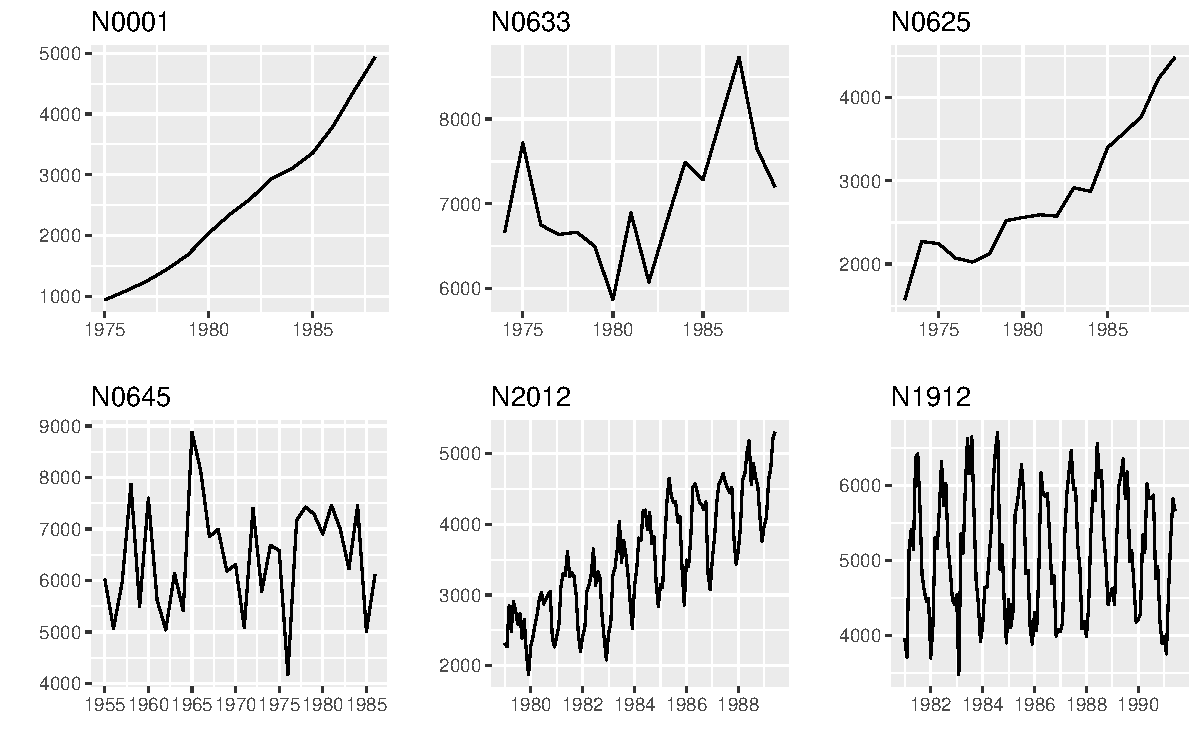
\includegraphics[width=\textwidth]{figure/fig1-1} 

}

\caption{Time-domain representation of time series}\label{fig:fig1}
\end{figure}

\begin{figure}

{\centering 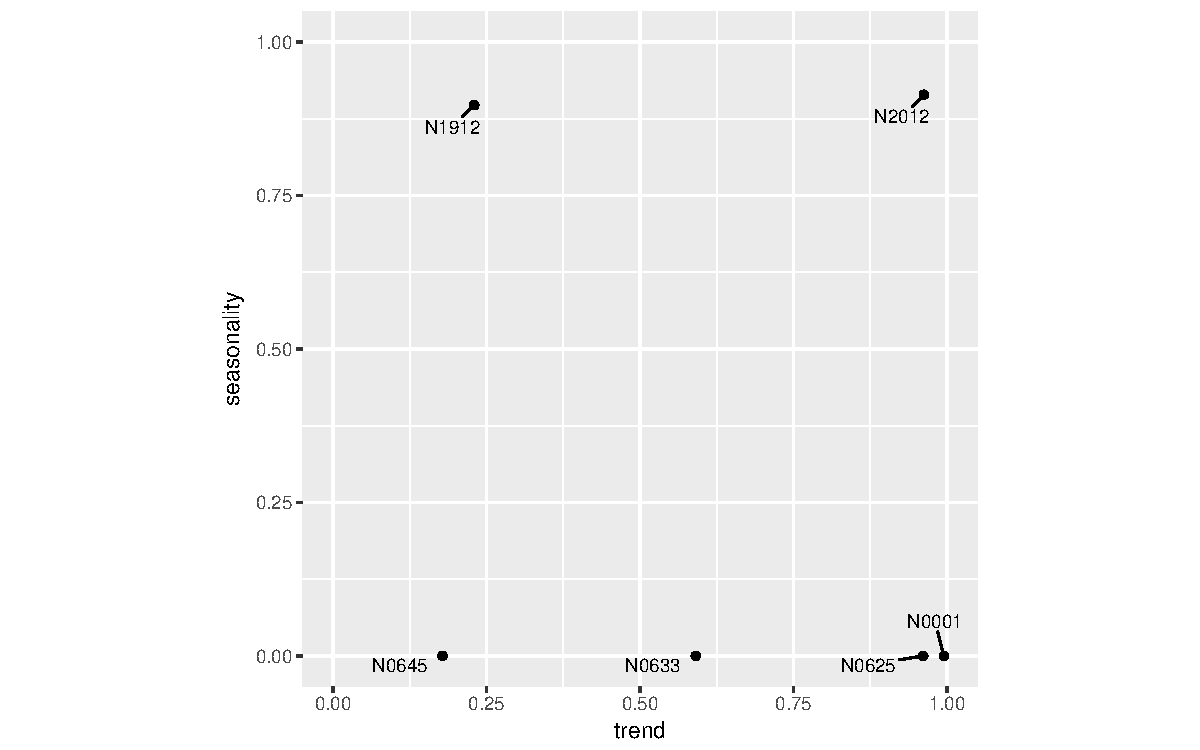
\includegraphics[width=0.7\linewidth]{figure/fig2-1} 

}

\caption{Feature-based representation of time series}\label{fig:fig2}
\end{figure}

The choice of the most appropriate set of features depends on both the nature of the time series being analysed, and the purpose of the analysis. In \autoref{Mcomp}, we study the time series from the M1 and M3 competitions \autocites{makridakis1982accuracy}{makridakis2000m3}, and we select features for the purpose of forecast-model selection. The M1 and M3 competitions involve time series of differing length, scale and other properties. We include length as one of our features, but the remaining features are independent of scale and asymptotically independent of the length of the time series (i.e., they are ergodic). As our main focus is forecasting, we select features which have discriminatory power in selecting a good model for forecasting.

\hypertarget{what-makes-features-useful-for-forecast-model-selection}{%
\subsection{What makes features useful for forecast-model selection?}\label{what-makes-features-useful-for-forecast-model-selection}}

\textcite{reid1972comparison} points out that the performance of forecasting methods changes according to the nature of the data. Exploring the reasons for these variations may be useful in selecting the most appropriate model. In response to the results of the M3 competition \autocite{makridakis2000m3}, similar ideas have been put forward by others. \textcite{hyndman2001s}, \textcite{lawrence2001s} and \textcite{armstrong2001s} argue that the characteristics of a time series may provide useful insights into which methods are most appropriate for forecasting.

Many time series forecasting techniques have been developed to capture specific characteristics of time series that are common in a particular discipline. For example, GARCH models were introduced to account for time-varying volatility in financial time series, and ETS models were introduced to handle the trend and seasonal patterns which are typical in quarterly and monthly sales data. An appropriate set of features should reveal the characteristics of the time series that are useful in determining the best forecasting method.

Several researchers have introduced rules for forecasting based on features \autocites{collopy1992rule}{adya2001automatic}{wang2009rule}. Most recently \textcite{kang2017visualising} applied principal component analysis to project a large collection of time series into a two dimensional feature space in order to visualize what makes a particular forecasting method perform well or not. The features they considered were spectral entropy, first-order auto-correlation coefficient, strength of trend, strength of seasonality, seasonal period and the optimal Box-Cox transformation parameter. They also proposed a method for generating new time series based on specified features.

\hypertarget{meta-learning-for-algorithm-selection}{%
\subsection{Meta-learning for algorithm selection}\label{meta-learning-for-algorithm-selection}}

John Rice was an early and strong proponent of the idea of meta-learning, which he called the algorithm selection problem (ASP) \autocite{rice1976}. The term \emph{meta-learning} started to appear with the emergence of the machine-learning literature. Rice's framework for algorithm selection is shown in \autoref{fig:rice} and comprises four main components. The problem space, \(P\), represents the data sets used in the study. The feature space, \(F\), is the range of measures that characterize the problem space \(P\). The algorithm space, \(A\), is a list of suitable candidate algorithms which can be used to find solutions to the problems in \(P\). The performance metric, \(Y\), is a measure of algorithm performance such as accuracy, speed, etc. A formal definition of the algorithm selection problem is given by \textcite{smith2009cross}, and repeated below.

\begin{quote}
\textbf{Algorithm selection problem}. For a given problem instance \(x \in P\), with features \(f(x) \in F\), find the selection mapping \(S(f(x))\) into algorithm space \(A\), such that the selected algorithm \(\alpha \in A\) maximizes the performance mapping \(y(\alpha(x)) \in Y\).
\end{quote}

\begin{figure}

{\centering 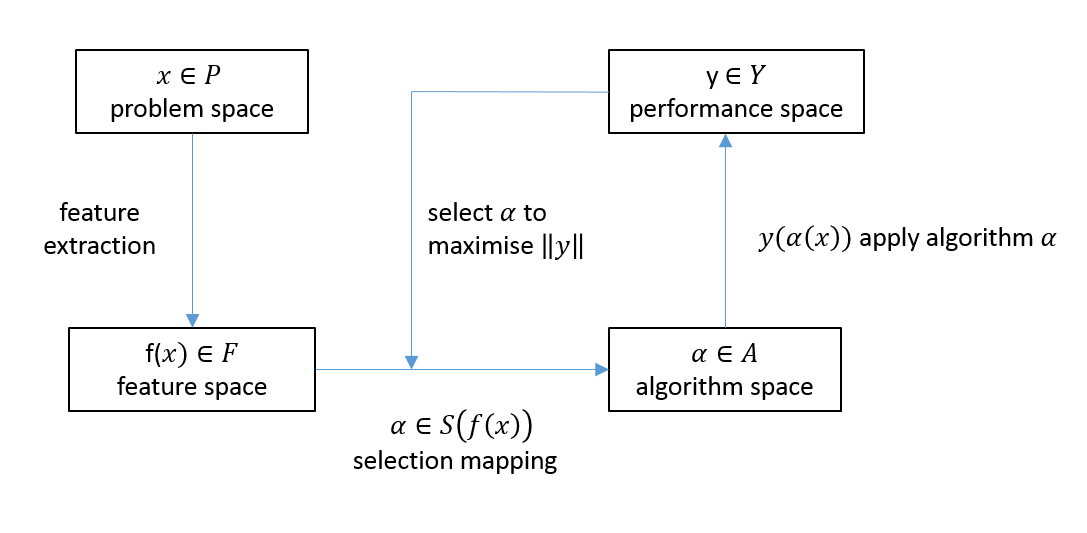
\includegraphics[width=0.8\linewidth]{figures/RiceFramework} 

}

\caption{Rice's framework for the Algorithm Selection Problem.}\label{fig:rice}
\end{figure}

The main challenge in ASP is to identify the selection mapping \(S\) from the feature space to the algorithm space. Even though Rice's framework articulates a conceptually rich framework, it does not specify how to obtain \(S\). This gives rise to the meta-learning approach.

\hypertarget{forecast-model-selection-using-meta-learning}{%
\subsection{Forecast-model selection using meta-learning}\label{forecast-model-selection-using-meta-learning}}

Selecting models for forecasting can be framed according to Rice's ASP framework.

\begin{quote}
\textbf{Forecast-model selection problem}. For a given time series \(x \in P\), with features \(f(x) \in F\), find the selection mapping \(S(f(x))\) into the algorithm space \(A\), such that the selected algorithm \(\alpha \in A\) minimizes forecast accuracy error metric \(y(\alpha(x)) \in Y\) on the test set of the time series.
\end{quote}

Existing methods differ with respect to the way they define the problem space (\(A\)), the features (\(F\)), the forecasting accuracy measure (\(Y\)) and the selection mapping (\(S\)).

\textcite{collopy1992rule} introduced 99 rules based on 18 features of time series, in order to make forecasts for economic and demographic time series. This work was extended by \textcite{armstrong2001s} to reduce human intervention.

\textcite{shah1997model} used the following features to classify time series: the number of observations, the ratio of the number of turning points to the length of the series, the ratio of number of step changes, skewness, kurtosis, the coefficient of variation, autocorrelations at lags 1--4, and partial autocorrelations at lag 2--4. Casting Shah's work in Rice's framework, we can specify: \(P=203\) quarterly series from the M1 competition \autocite{makridakis1982accuracy}; \(A=3\) forecasting methods, namely simple exponential smoothing, Holt-Winters exponential smoothing with multiplicative seasonality, and a basic structural time series model; \(Y=\) mean squared error for a hold-out sample. \textcite{shah1997model} learned the mapping \(S\) using discriminant analysis.

\textcite{prudencio2004meta} was the first paper to use the term ``meta-learning'' in the context of time series model selection. They studied the applicability of meta-learning approaches for forecast-model selection based on two case studies. Again using the notation above, we can describe their first case study with: \(A\) contained only two forecasting methods, simple exponential smoothing and a time-delay neural network; \(Y=\) mean absolute error; \(F\) consisted of 14 features, namely length, autocorrelation coefficients, coefficient of variation, skewness, kurtosis, and a test of turning points to measure the randomness of the time series; \(S\) was learned using the C4.5 decision tree algorithm. For their second study, the algorithm space included a random walk, Holt's linear exponential smoothing and AR models; the problem space \(P\) contained the yearly series from the M3 competition \autocite{makridakis2000m3}; \(F\) included a subset of features from the first study; and \(Y\) was a ranking based on error. Beyond the task of forecast-model selection, they used the NOEMON approach to rank the algorithms \autocite{kalousis1999noemon}.

\textcite{lemke2010meta} studied the applicability of different meta-learning approaches for time series forecasting. Their algorithm space \(A\) contained ARIMA models, exponential smoothing models and a neural network model. In addition to statistical measures such as the standard deviation of the de-trended series, skewness, kurtosis, length, strength of trend, Durbin-Watson statistics of regression residuals, the number of turning points, step changes, a predictability measure, nonlinearity, the largest Lyapunov exponent, and auto-correlation and partial-autocorrelation coefficients, they also used frequency domain based features. The feed forward neural network, decision tree and support vector machine approaches were considered to learn the mapping \(S\).

\textcite{wang2009rule} used a meta-learning framework to provide recommendations as to which forecast method to use to generate forecasts. In order to evaluate forecast accuracy, they introduced a new measure \(Y =\) \emph{simple percentage better (SPB)}, which calculates the forecasting accuracy of a method against the forecasting accuracy error of random walk model. They used a feature set \(F\) comprising nine features: strength of trend, strength of seasonality, serial correlation, nonlinearity, skewness, kurtosis, self-similarity, chaos and periodicity. The algorithm space \(A\) included eight forecast-models, namely, exponential smoothing, ARIMA, neural networks and random walk model; while the mapping \(S\) was learned using the C4.5 algorithm for building decision trees. In addition, they used SOM clustering on the features of the time series in order to understand the nature of time series in a two-dimensional setting.

The set of features introduced by \textcite{wang2009rule} was later used by \textcite{widodomodel} to develop a meta-learning framework for forecast-model selection. The authors further reduced the dimensionality of time series by performing principal component analysis on the features.

More recently, \textcite{kuck2016meta} proposed a meta-learning framework based on neural networks for forecast-model selection. Here, \(P = 78\) time series from the NN3 competition were used to build the meta-learner. They introduced a new set of features based on forecasting errors. The average symmetric mean absolute percentage error was used to identify the best forecast-models for each series. They classify their forecast-models in the algorithm space \(A\), comprising single, seasonal, seasonal-trend and trend exponential smoothing. The mapping \(S\) was learned using a feed-forward neural network. Further, they evaluated the performance of different sets of features for forecast-model selection.

\hypertarget{methodology}{%
\section{Methodology}\label{methodology}}

Our proposed FFORMS framework, presented in \autoref{fig:framework}, builds on this preceding research. The offline and online phases are shown in blue and red respectively. A classification algorithm (the meta-learner) is trained during the offline phase and is then used to select an appropriate forecast model for a new time series in the online phase.

\begin{figure}

{\centering 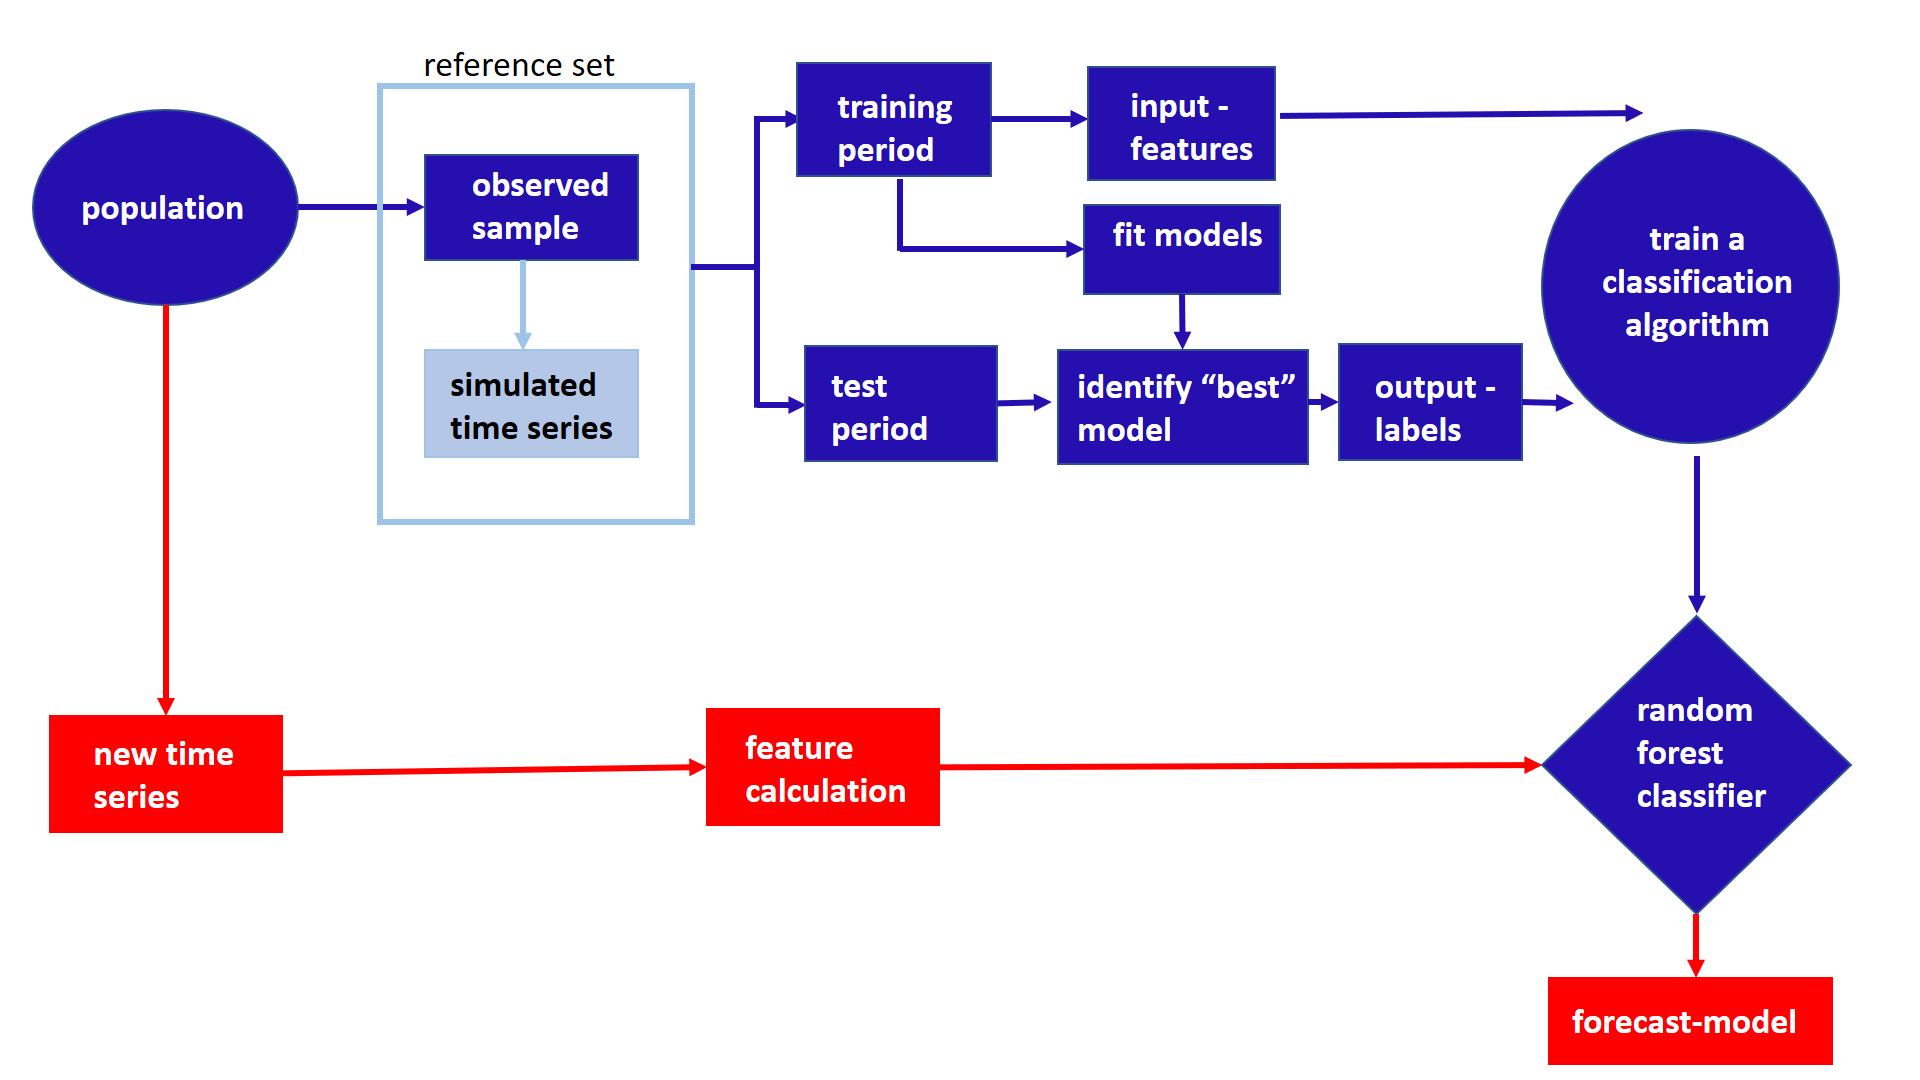
\includegraphics[width=\textwidth]{figures/framework} 

}

\caption{FFORMS (Feature-based FORecast-Model Selection) framework. The offline phase is shown in blue and the online phase in red.}\label{fig:framework}
\end{figure}

In order to train our classification algorithm, we need a large collection of time series which are similar to those we will be forecasting. We assume that we have an essentially infinite population of time series, and we take a sample of them in order to train the classification algorithm denoted as the ``observed sample''. The new time series we wish to forecast can be thought of as additional draws from the same population. Hence, any conclusions made from the classification framework refer only to the population from which the sample has been selected. We may call this the ``target population'' of time series. It is important to have a well-defined target population to avoid misapplying the classification rules. In practice, we may wish to augment the set of observed time series by simulating new time series similar to those in the assumed population (we provide details and discussion in Section \ref{simulatingseries} that follows). We denote the total collection of time series used for training the classifier as the ``reference set''.
Each time series within the reference set is split into a training period and a test period. From each training period we compute a range of time series features, and fit a selection of candidate models. The calculated features form the input vector to the classification algorithm. Using the fitted models, we generate forecasts and identify the ``best'' model for each time series based on a forecast error measure (e.g., MASE) calculated over the test period. The models deemed ``best'' form the output labels for the classification algorithm. The pseudo code for our proposed framework is presented in Algorithm \ref{alg:algo-lab} below. In the following sections, we briefly discuss aspects of the offline phase.

\begin{algorithm}[!ht]
  \caption{The FFORMS framework - Forecasting based on meta-learning. }
  \label{alg:algo-lab}
  \begin{algorithmic}[1]
    \Statex \textbf{Offline phase - train the classifier}
    \Statex \text{Given:}
    \Statex \hspace{1cm}$O=\{x_1, x_2, \dots,x_n\}:$ the collection of $n$ observed time series.
      \Statex \hspace{1cm}$L:$ the set of class labels (e.g.\ ARIMA, ETS, SNAIVE).
         \Statex \hspace{1cm}$F:$ the set of functions to calculate time series features.
         \Statex \hspace{1cm}$nsim:$ number of series to be simulated.
         \Statex \hspace{1cm}$B:$ number of trees in the random forest.
         \Statex \hspace{1cm}$k:$ number of features to be selected at each node.
     \Statex \text{Output:}
      \Statex \hspace{1cm}\text{FFORMS classifier}
      \Statex
     \Statex \textit{Prepare the reference set}
    \Statex For $i=1$ to $n$:
            \State Fit ARIMA and ETS models to $x_i$.
            \State Simulate $nsim$ time series from each model in step 1.
            \State The time series in $O$ and simulated time series in step 2 form the reference set $R=\{x_1, x_2, \dots,x_n, x_{n+1},\dots,x_N\}$ where $N = n + nsim$.
    \Statex
    \Statex \textit{Prepare the meta-data}
    \Statex For $j=1$ to $N$:
            \State Split $x_j$ into a training period and test period.
            \State Calculate features $F$ based on the training period.
            \State Fit $L$ models to the training period.
            \State Calculate forecasts for the test period from each model.
            \State Calculate forecast error measure over the test period for all models in $L$.
            \State Select the model with the minimum forecast error.
            \State Meta-data: input features (step 5), output labels (step 9).
     \Statex
    \Statex \textit{Train a random forest classifier}
            \State Train a random forest classifier based on the meta-data.
            \State {Random forest: the ensemble of trees $\{T_b\}_1^B$}.
    \Statex
     \Statex \textbf{Online phase - forecast a new time series}
    \Statex \text{Given:}
    \Statex \hspace{1cm}\text{FFORMS classifier from step 12} .
     \Statex \text{Output:}
      \Statex \hspace{1cm}\text{class labels for new time series $x_{new}$}.
  \State For $x_{new}$ calculate features $F$.
  \State Let $\hat{C_b}(x_{new})$ be the class prediction of the $b^{th}$ random forest tree. Then class label for $x_{new}$ is $\hat{C_{rf}}(x_{new})=majorityvote\{\hat{C_b}(x_{new})\}_1^B$.
   \end{algorithmic}
\end{algorithm}

\hypertarget{simulatingseries}{%
\subsection{Augmenting the observed sample with simulated time series}\label{simulatingseries}}

In practice, we may wish to augment the set of observed time series by simulating new time series similar to those in the assumed population. This process may be useful when the number of observed time series is too small to build a reliable classifier. Alternatively, we may wish to add more of some particular types of time series to the reference set in order to get a more balanced sample for the classification. In order to produce simulated series that are similar to those in the population, we consider two classes of data generating processes: exponential smoothing models and ARIMA models. Using the automated \texttt{ets} and \texttt{auto.arima} algorithms \autocite{forecast} we identify models, based on model selection criteria (such as AICc) and simulate multiple time series from the selected models within each model class. Assuming the models produce data that are similar to the observed time series ensures that the simulated series are similar to those in the population. As this is done in the offline phase of the algorithm the computational time in producing these simulated series is of no real consequence.

\hypertarget{input-features}{%
\subsection{Input: features}\label{input-features}}

Our proposed FFORMS algorithm requires features that enable identification of a suitable forecast model for a given time series. Therefore, the features used should capture the dynamic structure of the time series, such as trend, seasonality, autocorrelation, nonlinearity, heterogeneity, and so on. Furthermore, interpretability, robustness to outliers, scale and length independence should also be considered when selecting features for this classification problem. A comprehensive description of the features used in the experiment is presented in \autoref{feature}.

A feature of the proposed FFORMS framework is that its online phase is fast compared to the time required for implementing a typical model selection or cross-validation procedure. Therefore, we consider only features that can be computed rapidly, as this computation must be done during the online phase.

\hypertarget{output-labels}{%
\subsection{Output: labels}\label{output-labels}}

The task of the classification algorithm is to identify the ``best'' forecasting method for a given time series. It is not possible to train the classifier for all possible classes of models. However, we should consider enough possibilities so that the algorithm can be used for forecast-model selection with some confidence. The candidate models considered as labels will depend on the observed time series. For example, if we have only non-seasonal time series, and no chaotic features, we may wish to restrict the models to white noise, random walk, ARIMA and ETS processes. Even in this simple scenario, the number of possible models can be quite large.

Each candidate model considered is estimated strictly on the training period of each series in the reference set. Forecasts are then generated for the test period over which the chosen forecast accuracy measure is calculated. The model with the lowest forecast error measure over the test period is deemed ``best''.

This step is the most computationally intensive and time-consuming, as each candidate model has to be applied on each series in the reference set. However, as this task is done during the offline phase of the FFORMS framework, the time involved and computational cost associated are of no real significance and are completely controlled by the user. The more candidate models that are considered as labels, the more computational time is required; however the pay-off could be significant gains in forecast accuracy. \textcolor{black}{This is similar to other computationally intensive supervised learning method such as deep learning. The training process could take couple of days, but application could be done within few second even with your phone.}

\hypertarget{random-forest-algorithm}{%
\subsection{Random forest algorithm}\label{random-forest-algorithm}}

A random forest \autocite{breiman2001random} is an ensemble learning method that combines a large number of decision trees using a two-step randomization process. Let \((\bm{f}_1, z_1), (\bm{f}_2, z_2), \dots, (\bm{f}_N, z_N)\) represent the reference set, where input \(\bm{f}_i\) is an \(m\)-vector of features, output \(z_i\) corresponds to the class label of the \(i\)th time series, and \(N\) is the number of series in the reference set. Each tree in the forest is grown based on a bootstrap sample of size \(N\) from the reference set. At each node of the tree, randomly select \(k < m\) features from the full set of features. The best split is selected among those \(k\) features. The split which results in the most homogeneous subnodes is considered the best split. Various measures have been introduced to evaluate the homogeneity of subnodes, such as classification error rate, the Gini index and cross entropy \autocite{friedman2001elements}. In this study, we use the Gini index to evaluate the homogeneity of a particular split. The trees are grown to the largest extent possible without pruning. To determine the class label for a new instance, features are calculated and passed down the trees. Then each tree gives a prediction and the majority vote over all individual trees leads to the final decision. In this work, we have used the randomForest package \autocites{liaw2002randomforest}{rfpkg} which implements the Fortran code for random forest classification by \textcite{breiman2004random}.

\hypertarget{Mcomp}{%
\section{Application to the M competition data}\label{Mcomp}}

To test how well our proposed framework can identify suitable models for forecasting, we use the yearly, quarterly and monthly series from the M1 \autocite{makridakis1982accuracy} and M3 competitions \autocite{makridakis2000m3}. The R package Mcomp \autocite{hyndmanmcomp} provides the data for both these. We run two experiments. In the first experiment, we treat the time series from the M1 competition as the \emph{observed sample} and the time series from the M3 competition as the \emph{new time series} to be forecast. We reverse the sets in the second experiment, treating the M3 data as the \emph{observed sample} and the M1 data as the \emph{new time series}. The experimental set-ups are summarised in \autoref{tbl:Mcomps}. These allow us to compare our results with published forecast accuracy results for each of these competitions.

\begin{table}[!htp]
\centering\footnotesize
\caption{The number of series and their sources used in the two forecast experiments.}
\label{tbl:Mcomps}
\begin{tabular}{lcrrrc@{\hspace*{0.3cm}}crrr}
\toprule
  & \multicolumn{4}{c}{Experiment 1} & &\multicolumn{4}{c}{Experiment 2} \\
  & Source  & Yearly & Quarterly  & Monthly && Source & Yearly & Quarterly & Monthly \\
\cline{2-5}\cline{7-10}\\[-0.25cm]
Observed series & M1 & 181 & 203 & 617  && M3 & 645 & 756 & 1428 \\
New series      & M3 & 645 & 756 & 1428 && M1 & 181 & 203 & 617 \\
\bottomrule
\end{tabular}
\end{table}

In each experiment, we fit ARIMA and ETS models to the full length of each series in the corresponding \emph{observed samples} using the \texttt{auto.arima} and \texttt{ets} functions in the forecast package. From each model fitted to the annual and quarterly data, we simulate a further 1000 series for augmenting the reference set. For the monthly time series, we simulate a further 100 series (in order to save time in the offline calculation process). The lengths of the simulated series are set to be equal to the lengths of the series on which these are based on.

As shown in \autoref{fig:framework}, the task of constructing the meta-database contains two main components: (i) identification of the candidate forecast models as output labels and (ii) computation of features.

\hypertarget{sec:labels}{%
\subsection{Identifying output labels}\label{sec:labels}}

The candidate models we consider as class labels for the annual series are:

\begin{enumerate}
\def\labelenumi{(\alph{enumi})}
\tightlist
\item
  White noise (WN)
\item
  AR/MA/ARMA
\item
  ARIMA;
\item
  Random walk with drift (RWD);
\item
  Random walk (RW);
\item
  Theta;
\item
  Exponential Smoothing Model (ETS) without trend and seasonal components;
\item
  ETS with trend component and without seasonal component;
\item
  ETS with damped trend component and without seasonal component;
\end{enumerate}

In addition to the above nine labels, we further include the following six class labels for both quarterly and monthly data:

\begin{enumerate}
\def\labelenumi{(\alph{enumi})}
\setcounter{enumi}{9}
\tightlist
\item
  STL-AR;
\item
  ETS with trend and seasonal components
\item
  ETS with damped trend and seasonal components
\item
  ETS with seasonal components and without trend component
\item
  SARIMA
\item
  Seasonal naive method.
\end{enumerate}

Most of these are self-explanatory labels based on models implemented in the forecast package using the default settings.

STL-AR refers to forecasts based on an STL decomposition applied to the time series, then an AR model is used to forecast the seasonally adjusted data, while the seasonal naive method is used to forecast the seasonal component. The two sets of forecasts are then combined to provide forecasts on the original time scale \autocite{hyndman2014forecasting}.

For each series in the reference set, all candidate models are estimated using the training period, and forecasts are generated for the whole of the test period \textcolor{black}{(based on "fixed origin" evaluation)} as set by the competitions. The model corresponding to the smallest MASE \autocite{hyndman2006another} calculated over the test period is selected as the ``best model'' and forms the \emph{output label} for that series.

\hypertarget{sec:features}{%
\subsection{Feature computation process}\label{sec:features}}

We use a set of 25 features for yearly data and a set of 30 features for seasonal data. Some of these are taken from previous studies \autocites{wang2009rule}{hyndman2015large}{kang2017visualising}, and we have also added new features that we believe provide some useful information. Each feature can be computed rapidly, thus making the online phase of our algorithm extremely fast. The features are summarized in \autoref{feature}, and fully described in the Appendix.

Correlation matrices for all the features calculated from the reference sets of each of the experiments are presented in \autoref{fig:cormatplots}. The variability in the correlations reflects the diversity of the selected features. In other words, the features we have employed seem to capture different characteristics of the time series. Furthermore, the structure of the correlation matrices across the same frequencies of the two experiments seem to be fairly similar. This sends a strong signal that the M1 and M3 collections of time series may have similar feature spaces.

\begin{table}[!htp]
\centering\footnotesize\tabcolsep=0.12cm
\caption{Features used for selecting a forecast-model (see Appendix A for details).}
\label{feature}
\begin{tabular}{llp{8,8cm}cc}
\toprule
\multicolumn{2}{c}{Feature} & Description & Non-seasonal & Seasonal\\
\midrule
1  & T              & length of time series                                                                   & \yes  & \yes \\
2  & trend          & strength of trend                                                                       & \yes  & \yes\\
3  & seasonality    & strength of seasonality                                                                 & -     & \yes \\
4  & linearity      & linearity                                                                               & \yes  & \yes \\
5  & curvature      & curvature                                                                               & \yes  & \yes \\
6  & spikiness      & spikiness                                                                               & \yes  & \yes \\
7  & e\_acf1        & first ACF value of remainder series                                                     & \yes  & \yes \\
8  & stability      & stability                                                                               & \yes  & \yes \\
9  & lumpiness      & lumpiness                                                                               & \yes  & \yes \\
10 & entropy        & spectral entropy                                                                        & \yes  & \yes \\
11 & hurst          & Hurst exponent                                                                          & \yes  & \yes \\
12 & nonlinearity   & nonlinearity                                                                            & \yes\ & \yes \\
13 & alpha          & ETS(A,A,N) $\hat\alpha$                                                                 & \yes  & \yes \\
14 & beta           & ETS(A,A,N) $\hat\beta$                                                                  & \yes  & \yes\\
15 & hwalpha        & ETS(A,A,A) $\hat\alpha$                                                                 & -     & \yes \\
16 & hwbeta         & ETS(A,A,A) $\hat\beta$                                                                  & -     & \yes \\
17 & hwgamma        & ETS(A,A,A) $\hat\gamma$                                                                 & -     & \yes \\
18 & ur\_pp         & test statistic based on Phillips-Perron test                                            & \yes  & - \\
19 & ur\_kpss       & test statistic based on KPSS test                                                       & \yes  & - \\
20 & y\_acf1        & first ACF value of the original series                                                  & \yes  & \yes \\
21 & diff1y\_acf1   & first ACF value of the differenced series                                               & \yes  & \yes \\
22 & diff2y\_acf1   & first ACF value of the twice-differenced series                                         & \yes  & \yes \\
23 & y\_acf5        & sum of squares of first 5 ACF values of original series                                 & \yes  & \yes \\
24 & diff1y\_acf5   & sum of squares of first 5 ACF values of differenced series                              & \yes  & \yes \\
25 & diff2y\_acf5   & sum of squares of first 5 ACF values of twice-differenced series                        & \yes  & \yes \\
26 & seas\_acf1     & autocorrelation coefficient at first seasonal lag                                       & -     & \yes \\
27 & sediff\_acf1   & first ACF value of seasonally-differenced series                                        & -     & \yes\\
28 & sediff\_seasacf1 & ACF value at the first seasonal lag of seasonally-differenced series                    & -     & \yes \\
29 & sediff\_acf5   & sum of squares of first 5 autocorrelation coefficients of seasonally-differenced series & -     & \yes \\
30 & seas\_pacf  & partial autocorrelation coefficient at first seasonal lag                      & -  & \yes \\
31 & lmres\_acf1    & first ACF value of residual series of linear trend model                                & \yes  & - \\
32 & y\_pacf5       & sum of squares of first 5 PACF values of original series                                & \yes  & \yes \\
33 & diff1y\_pacf5  & sum of squares of first 5 PACF values of differenced series                             & \yes  & \yes \\
34 & diff2y\_pacf5  & sum of squares of first 5 PACF values of twice-differenced series                       & \yes  & \yes \\

\bottomrule
 \end{tabular}
\end{table}

\begin{figure}

{\centering 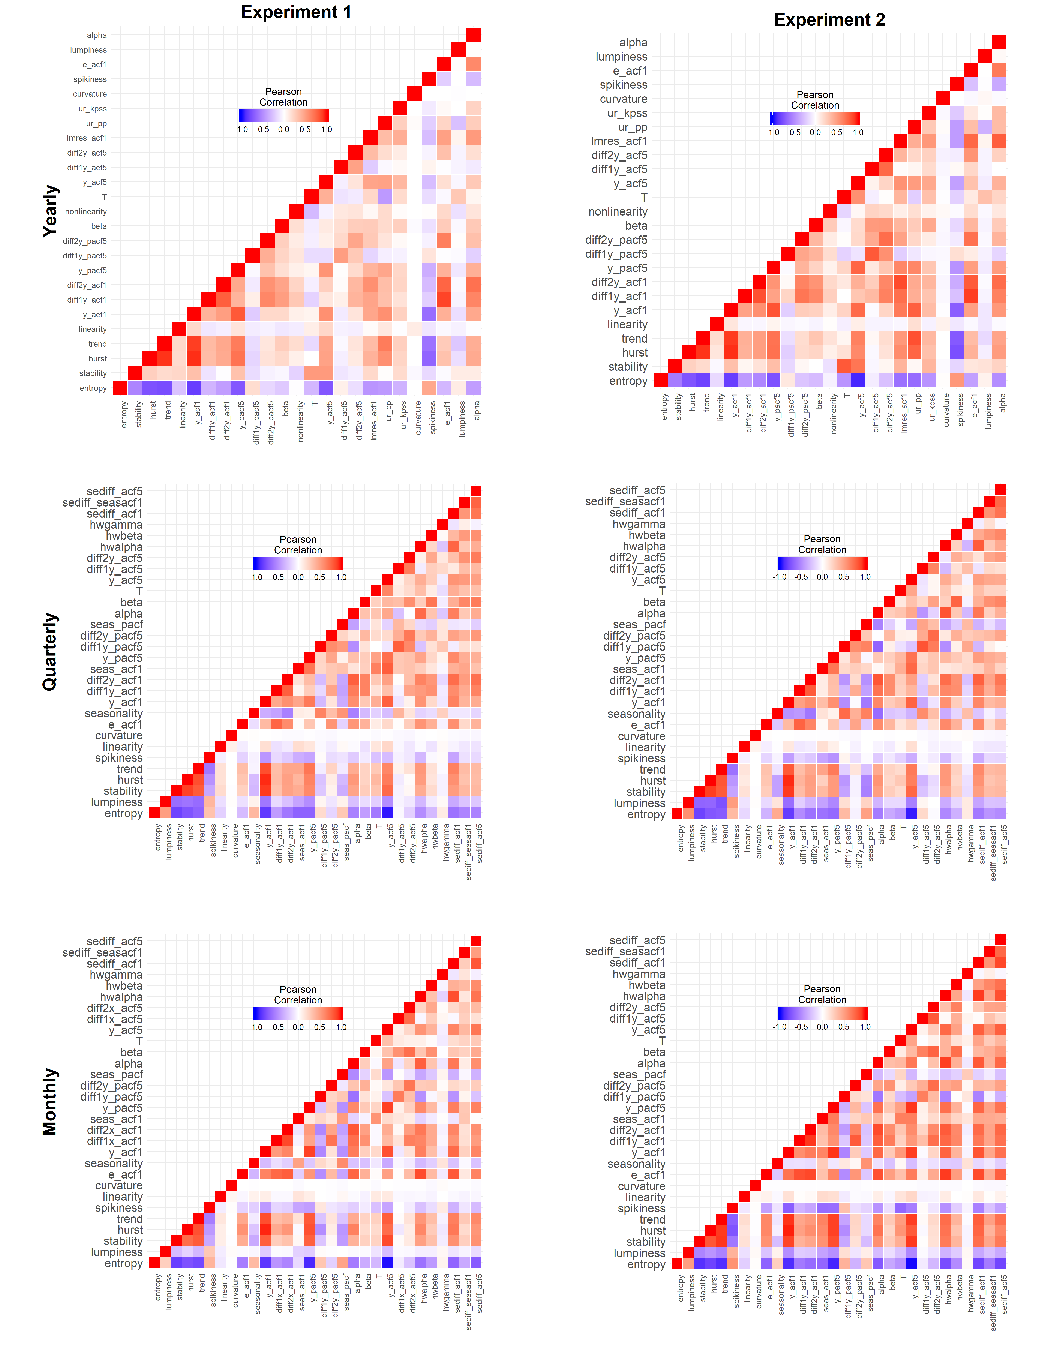
\includegraphics[width=\textwidth]{figure/cormatplots-1} 

}

\caption{ Correlation matrix plots for the reference sets.}\label{fig:cormatplots}
\end{figure}

\hypertarget{model-calibration}{%
\subsection{Model calibration}\label{model-calibration}}

\textcolor{black}{This is a multi-class classification task, with predictors = features, and outcome = categorical variable with all possible forecast models as its class label. In particular, an instance is a tuple $(f_{i1}, f_{i2}, \dots, f_{im}, z_i)$, where predictors = $(f_{i1}, f_{i2}, \dots, f_{im})$ is a vector of $m$ number of features which becomes input to our algorithm and outcome is $z_i$, the "best" forecast model. An example of instance is $(0.51, 0.12, \dots, 3.1, SARIMA)$.}
The random forest (RF) algorithm is highly sensitive to class imbalance \autocite{breiman2001random}, and our reference set is unbalanced: some classes contain significantly more cases than other classes. The degree of class imbalance is reduced to some extent by augmenting the observed sample with the simulated time series. We consider three approaches to address the class imbalance in the data: (1) incorporating class priors into the RF classifier; (2) using the balanced RF algorithm introduced by \textcite{chen2004using}; and (3) re-balancing the reference set with down-sampling. In down-sampling, the size of the reference set is reduced by down-sampling the larger classes so that they match the smallest class in size; this potentially discards some useful information. Comparing the results, the balanced RF algorithm and RF with down-sampling did not yield satisfactory results. We therefore only report the results obtained by the RF built on unbalanced data (RF-unbalanced) and the RF with class priors (RF-class priors). The RF algorithms are implemented by the randomForest R package \autocites{liaw2002randomforest}{rfpkg}. The class priors are introduced through the option \texttt{classwt}. We use the reciprocal of class size as the class priors. The number of trees \texttt{ntree} is set to 1000, and the number of randomly selected features \texttt{k} is set to be one third of the total number of features available.

Our aim is different from most classification problems in that we are not interested in accurately predicting the class, but in finding the best possible forecast model. It is possible that two models produce almost equally accurate forecasts, and therefore it is not important whether the classifier picks one model over the other. Therefore we report the forecast accuracy obtained from the FFORMS framework, rather than the classification accuracy.

\hypertarget{sec:results}{%
\subsection{Summary of the main results}\label{sec:results}}

We build separate RF classifiers for yearly data, quarterly data and monthly data. For the second experiment (for which data from the M3 competition are the observed series), in the case of yearly and quarterly data we take a subset of the simulated time series when training the RF-unbalanced and RF-class priors, to reduce the size of the reference set (these are shown in yellow in the figures that follow). The subsets are selected randomly according to the proportions of output labels in the observed samples. This ensures that our reference set shares similar characteristics to the observed sample.

We use principal component analysis to visualize the feature-spaces of the different time series collections. We compute the principal components projection using the features in the observed sample, and then project the simulated time series and the new time series using the same projection. The results are shown in Figures \ref{fig:exp1pca}--\ref{fig:exp2pca}, where the first three principal components are plotted against each other. Figure \ref{fig:exp1pca} refers to Experiment 1 and Figure \ref{fig:exp2pca} to Experiment 2. The points on each plot represent individual time series. In each figure the first column of plots refers to the yearly data, the middle column to the quarterly data and the last column to the monthly data. The plots show that the first three principal components explain 62.5\%, 62.4\% and 58.9\% of the total variation in the yearly, quarterly and monthly M1 data and 62.2\% 64.7\% and 66.0\% of the total variation in the yearly, quarterly and monthly M3 data.

\begin{figure}

{\centering 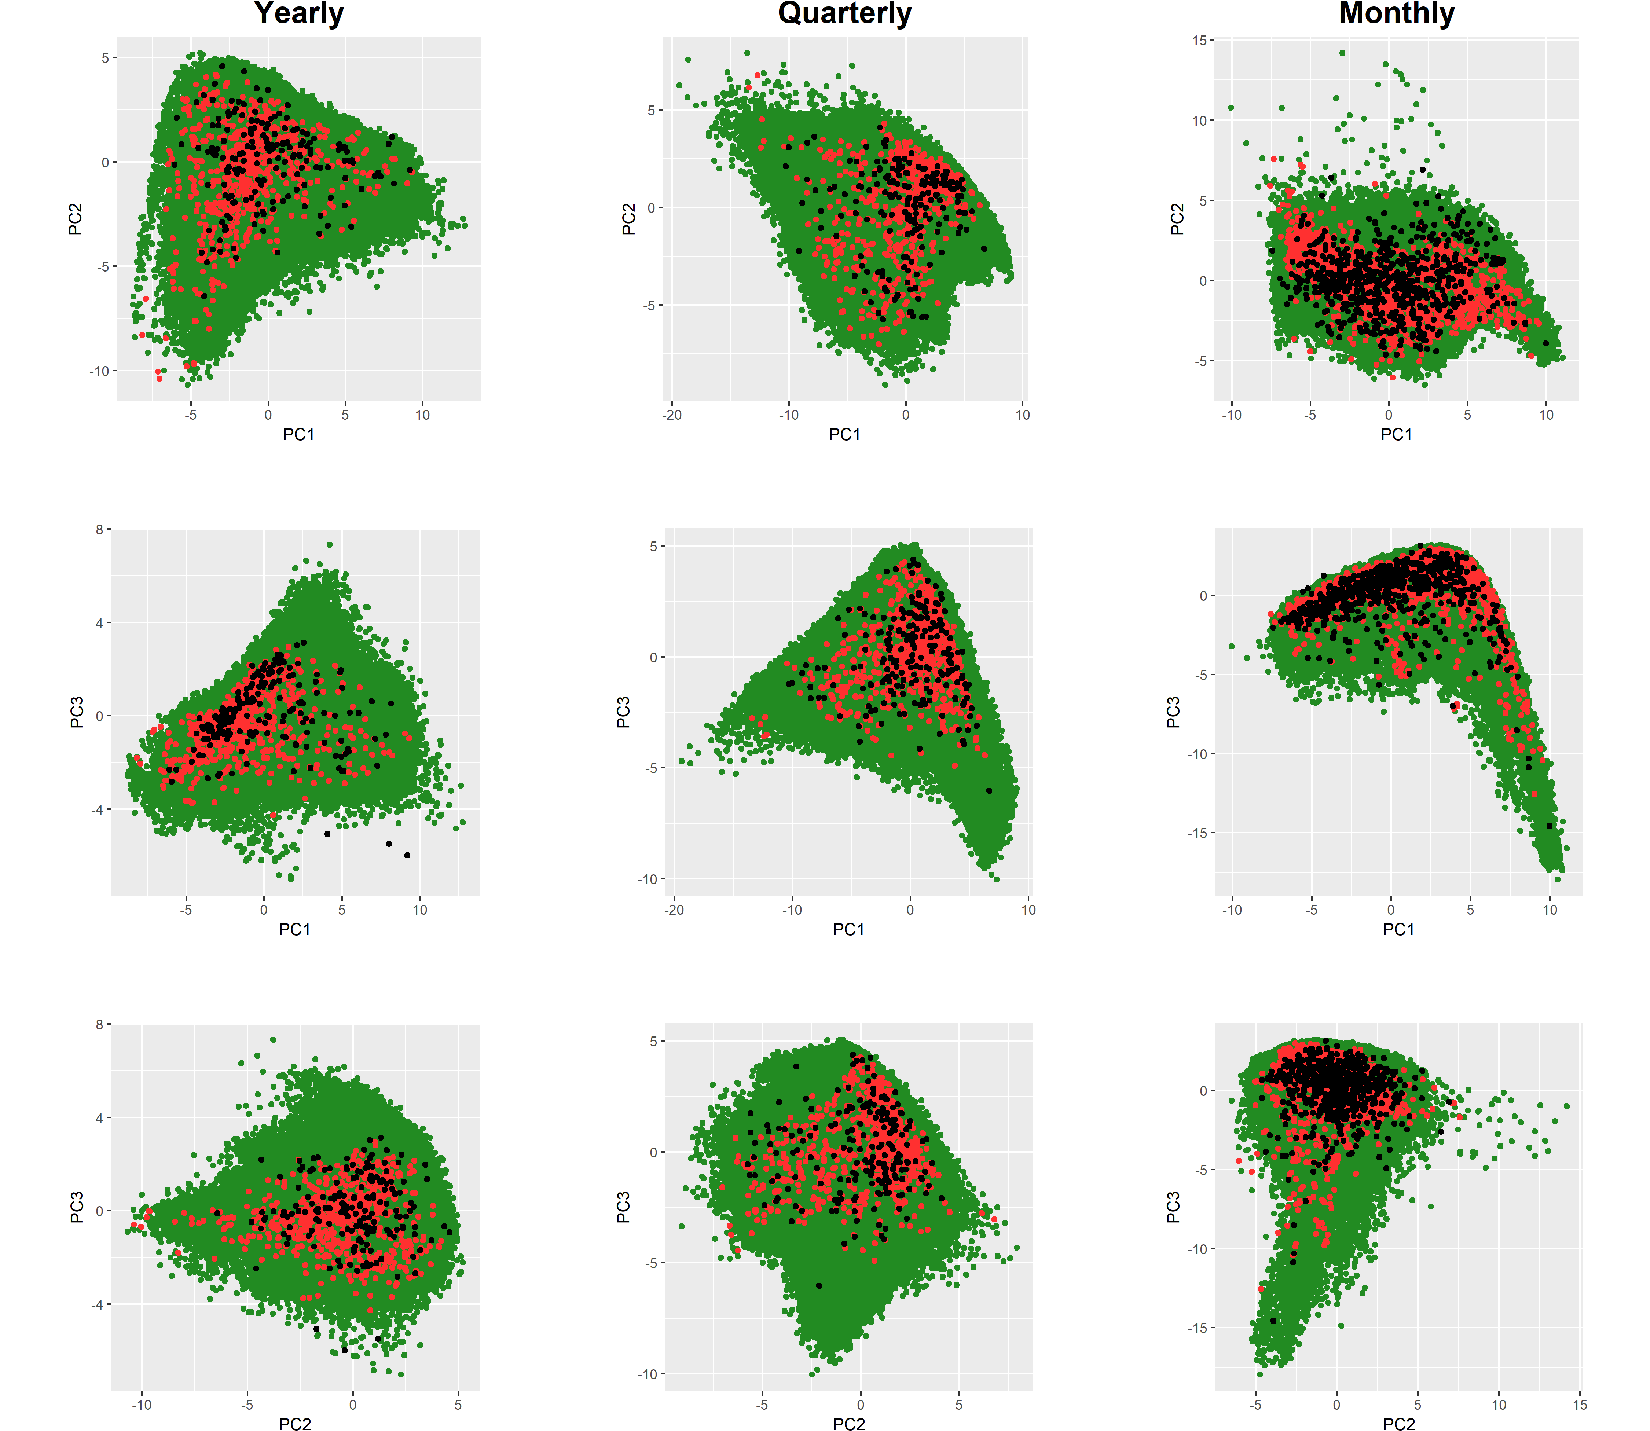
\includegraphics[width=\textwidth]{figure/exp1pca-1} 

}

\caption{Experiment 1: Distribution of time series in the PCA space. Distribution of yearly series are shown in the first column, distribution of quarterly series are shown in the second column, and the distribution of monthly series are shown in the third column. On each graph, green indicates simulated time series, black indicates observed time series, while orange denotes new time series.}\label{fig:exp1pca}
\end{figure}

\begin{figure}

{\centering 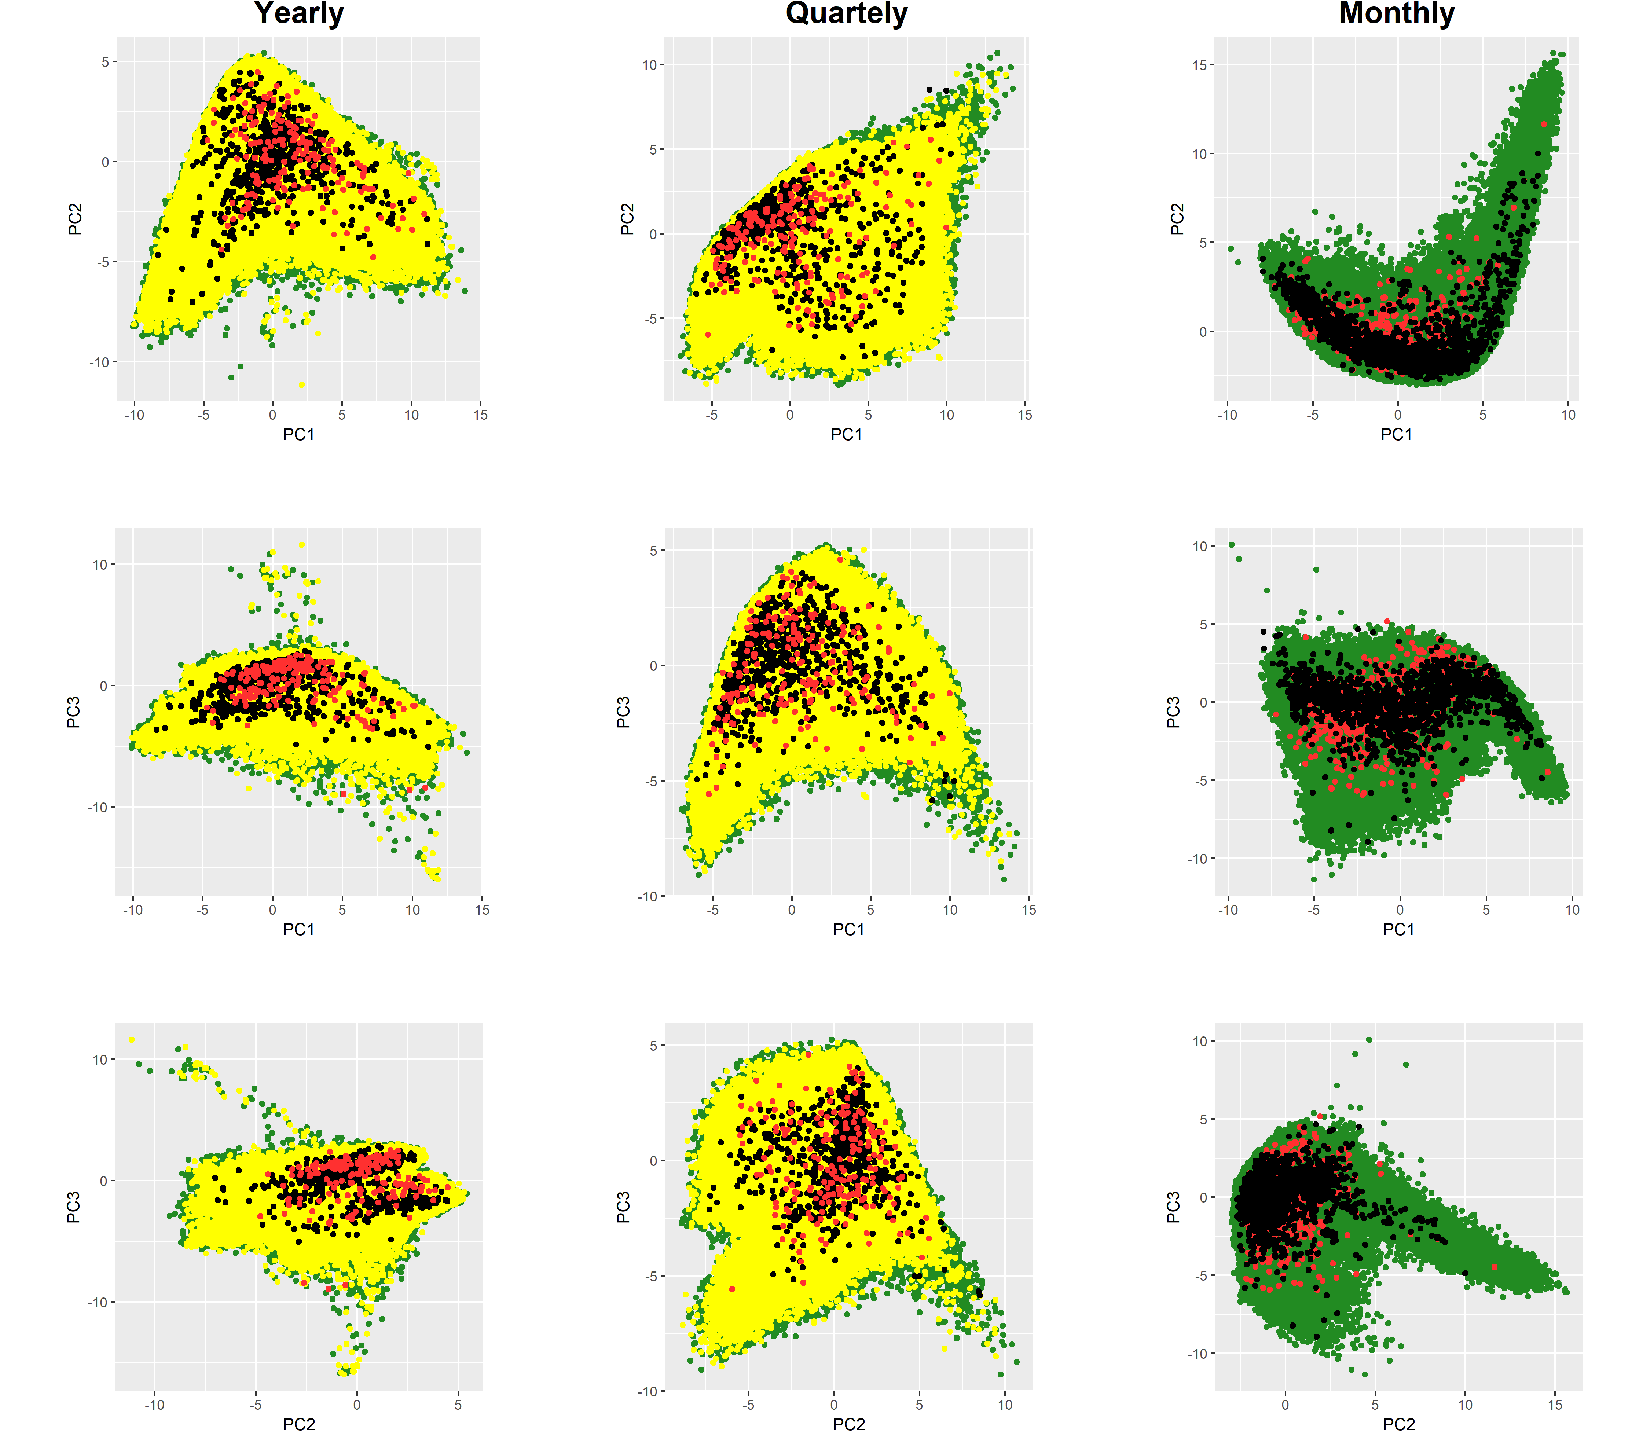
\includegraphics[width=\textwidth]{figure/exp2pca-1} 

}

\caption{Experiment 2: Distribution of time series in the PCA space. Distribution of yearly series are shown in the first column, distribution of quarterly series are shown in the second column, and the distribution of monthly series are shown in the third column. On each graph, green indicates simulated time series, yellow shows a subset of simulated time series, black indicates observed time series, while orange denotes new time series.}\label{fig:exp2pca}
\end{figure}

The plots show that the distribution of the observed time series over the PCA space (represented by the black dots) is very similar to that of the new time series (represented by the orange dots). More importantly, we see that the distribution of the simulated time series (represented by the green dots and yellow dots - the yellow dots are a subset of the simulated series as mentioned above) clearly nests and fills in the space of the new time series. Further, in both experiments, all the \emph{observed time series} fall within the space of all simulated data. This strongly indicates that we have not reduced the feature diversity from the observed sample. By augmenting the observed series with simulated time series, we have been able to increase the diversity and evenness of the feature space in the reference sets.

We compare the accuracy of the forecasts generated from the FFORMS framework to the following commonly-used forecasting methods:

\begin{enumerate}
\def\labelenumi{\arabic{enumi}.}
\tightlist
\item
  automated ARIMA algorithm of \textcite{Hyndman2008};
\item
  automated ETS algorithm of \textcite{Hyndman2008};
\item
  Random walk with drift (RWD);
\item
  Random walk model (RW);
\item
  White noise process (WN);
\item
  Theta method;
\item
  STL-AR method (for seasonal data);
\item
  seasonal naive (for seasonal data).
\end{enumerate}

The automated ARIMA and ETS algorithms are implemented using the \texttt{auto.arima} and \texttt{ets} functions available in the forecast package in R. Each method is implemented on the training period of the new series and forecasts are computed for the full length of the test period. This follows closely the forecast evaluation process implemented in the M1 and M3 forecasting competitions. The MASE is computed for each forecast horizon, by averaging the absolute scaled forecast errors across all series. The rank is calculated by averaging the ranks of each competing method across all forecast horizons and series. The results are presented in Table \ref{masetab}. \textcolor{black}{The associated box-and-whisker plots are shown in Figures}
\ref{fig:yearlybox} \textcolor{black}{through} \ref{fig:monthlybox} \textcolor{black}{in Appendix B.} The lowest MASE and average rank values corresponding to the best performing method are presented in bold font.

\begin{table}[!htbp]
\centering\footnotesize
\centering
\caption{MASE values calculated over the new series for Experiments 1 and 2.}
\label{masetab}
\begin{tabular}{lrrrrrrrrrrr}
\toprule
                     &                              \multicolumn{ 5}{c}{Experiment 1: new series M3} &            &                              \multicolumn{ 5}{c}{Experiment 2: new series M1} \\\cmidrule(lr){2-6} \cmidrule(lr){8-12}
                     &                                    \multicolumn{ 5}{c}{Yearly} &            &                                    \multicolumn{ 5}{c}{Yearly} \\
                     &   $h=1$    &    $1-2$   &     $1-4$  &     $1-6$  &      Rank  &            &     $h=1$  &    $1-2$   &     $1-4$  &     $1-6$  &   Rank \\\cmidrule(lr){2-6} \cmidrule(lr){8-12}
RF-unbalanced        &       1.06 &       1.40 &       2.17 &       2.82 &       3.50 &            & {\bf 0.98} & {\bf 1.40} &       {\bf 2.43} &       3.39 &        {\bf 1.50} \\
RF-class priors      & 1.04 &       1.38 &       2.15 &       2.79 &       2.50 &            &       1.01 &       {\bf 1.40} & {\bf 2.43} & {\bf 3.38} & {\bf 1.50} \\
auto.arima           &       1.11 &       1.48 &       2.28 &       2.96 &       5.83 &            &       1.06 &       1.47 &       2.51 &       3.47 &       3.33 \\
ets                  &       1.09 &       1.44 &       2.20 &       2.86 &       4.67 &            &       1.12 &       1.59 &       2.72 &       3.77 &       5.00 \\
WN                   &       6.54 &       6.91 &       7.48 &       8.07 &       9.00 &            &       6.38 &       7.08 &       8.59 &      10.01 &       8.00 \\
RW                   &       1.24 &       1.68 &       2.48 &       3.17 &       8.00 &            &       1.35 &       2.00 &       3.50 &       4.89 &       7.00 \\
RWD                  & {\bf 1.03} & {\bf 1.36} & {\bf 2.05} & {\bf 2.63} & {\bf 1.00} &            &       1.04 &       1.44 &       2.51 &       3.49 &       3.67 \\
Theta                &       1.12 &       1.47 &       2.18 &       2.77 &       3.50 &            &       1.15 &       1.70 &       3.00 &       4.19 &       6.00 \\\cmidrule(lr){2-6} \cmidrule(lr){8-12}
           &                                 \multicolumn{ 5}{c}{Quarterly} &            &                                 \multicolumn{ 5}{c}{Quarterly} \\
                     &    $h=1$   &    $1-4$   &     $1-6$  &     $1-8$  &      Rank  &            &     $h=1$  &    $1-4$   &     $1-6$  &     $1-8$  &   Rank \\\cmidrule(lr){2-6} \cmidrule(lr){8-12}
RF-unbalanced        &       0.59 & {\bf 0.81} & {\bf 0.97} &       1.12 & {\bf 2.25} &            & {\bf 0.74} & {\bf 1.08} & {\bf 1.35} & {\bf 1.57} & {\bf 1.00} \\
RF-class priors      &       0.59 & 0.82 &       {\bf 0.97} &       1.13 &  3.13 &            &       0.76 &       1.12 &       1.40 &       1.62 &       2.63 \\
auto.arima           &       0.59 &       0.85 &       1.02 &       1.19 &       4.75 &            &       0.78 &       1.17 &       1.50 &       1.74 &       5.25 \\
ets                  & {\bf 0.56} &       0.82 &       0.99 &       1.17 &       3.75 &            &       0.78 &       1.11 &       1.42 &       1.66 &       3.00 \\
WN                   &       3.25 &       3.59 &       3.70 &       3.87 &      10.00 &            &       3.97 &       4.27 &       4.45 &       4.64 &      10.00 \\
RW                   &       1.14 &       1.16 &       1.32 &       1.46 &       7.00 &            &       0.97 &       1.35 &       1.67 &       1.95 &       7.50 \\
RWD                  &       1.20 &       1.17 &       1.36 &       1.47 &       6.50 &            &       0.95 &       1.26 &       1.56 &       1.81 &       5.38 \\
STL-AR               &       0.70 &       1.27 &       1.60 &       1.91 &       8.34 &            &       0.96 &       1.63 &       2.05 &       2.43 &       8.63 \\
Theta                &       0.62 &       0.83 &       {\bf 0.97} & {\bf 1.11} &  2.50 &            &       0.79 &       1.13 &       1.42 &       1.67 &       3.88 \\
Snaive               &       1.11 &       1.09 &       1.30 &       1.43 &       6.75 &            &       1.52 &       1.56 &       1.87 &       2.08 &       7.75 \\\cmidrule(lr){2-6} \cmidrule(lr){8-12}
           &                                   \multicolumn{ 5}{c}{Monthly} &            &                                   \multicolumn{ 5}{c}{Monthly} \\
                     &    $h=1$ &    $1-6$   &     $1-12$ &    $1-18$  &   Rank     &            &   $h=1$  &    $1-6$   &    $1-12$  &    $1-18$  &   Rank \\\cmidrule(lr){2-6} \cmidrule(lr){8-12}
RF-unbalanced        &       0.60 &       0.68 &       0.76 &       0.87 &       3.22 &            &       0.61 &       0.76 & {\bf 0.90} & {\bf 1.03} &       {\bf 1.77} \\
RF-class priors      &       0.60 &       0.67 & 0.75 & {\bf 0.86} &       {\bf 2.00} &            &       0.60 &       {\bf 0.75} &       0.92 &       1.06 &        2.83 \\
auto.arima           &      {\bf 0.55 }&      {\bf 0.64} &      {\bf 0.74} &       0.87 &       2.83 &            &       0.60 &       0.76 &       0.96 &       1.12 &       4.94 \\
ets                  & {\bf 0.55} & {\bf 0.64} & {\bf 0.74} &       {\bf 0.86} & 2.72 &            &      {\bf 0.59} &       0.76 &       0.93 &       1.07 &       3.44 \\
WN                   &       2.01 &       2.08 &       2.15 &       2.27 &      10.00 &            &       1.93 &       2.09 &       2.18 &       2.28 &      10.00 \\
RW                   &       0.84 &       0.97 &       1.04 &       1.17 &    8.03 &            &       1.05 &       1.24 &       1.33 &       1.47 &      7.25 \\
RWD                  &       0.84 &       0.96 &       1.02 &       1.14 &       6.89 &            &       1.06 &       1.27 &       1.39 &       1.55 &      8.61 \\
STL-AR               &       0.64 &       0.81 &       1.04 &       1.27 &       7.89 &            &       0.63 &       0.91 &       1.17 &       1.39 &       7.38 \\
Theta                &       0.58 &       0.67 &       0.77 &       0.89 &       4.22 &            & 0.61 & {\bf 0.75} &       0.92 &       1.04 & 2.27 \\
Snaive               &       0.95 &       0.97 &       0.99 &       1.15 &       7.19 &            &       1.06 &       1.11 &       1.14 &       1.31 &       6.47 \\
\bottomrule
\end{tabular}
{\raggedright Note: $h$ is the length of the forecast horizon. \par}
\end{table}

In general, our proposed FFORMS meta-learning algorithm performs quite well in both experimental settings. It consistently ranks in the top most accurate forecasting methods for forecasting both the M1 and the M3 series and most often ranks as the most accurate method. For yearly data, FFORMS ranks best for forecasting the M1 data in experiment 2 and second (to the random walk with drift) in forecasting the M3 data. For quarterly data, FFORMS ranks as the most accurate in both experiments. For monthly data, FFORMS seems to perform best for the longer horizons in both experimental settings. It also seems to be competitive for the shorter horizons with the three methods (\texttt{auto.arima}, \texttt{ets} and theta) that perform best. Comparing the results across the two experimental settings, it seems that using the FFORMS algorithm achieves marginally better results in experiment 2. Hence, this indicates that the meta-learning algorithm benefits from being trained on the larger observed sample of time series (M3 series) while forecasting a smaller new set (M1 series).

\hypertarget{discussion}{%
\section{Discussion and conclusions}\label{discussion}}

In this paper we have proposed a novel framework for forecast-model selection using meta-learning based on time series features. Our proposed FFORMS algorithm uses the knowledge of the past performance of candidate forecast models on a collection of time series in order to identify the best forecasting method for a new series. We have shown that the method almost always performs better than common benchmark methods, and in many cases better than the best-performing methods from both the M1 and the M3 forecasting competitions. Although we have illustrated the method using the M1 and M3 competition data, the framework is general and can be applied to any large collection of time series.

A major advantage of the FFORMS framework is that the classifier is trained offline and selecting a forecasting model for a new time series is as fast as calculating a set of features and passing these to the pretrained classifier. Therefore, unlike traditional model selection strategies or cross-validation processes, our proposed framework can be used to accurately forecast very large collections of time series requiring almost instant forecasts.

In addition to our new FFORMS framework, we have also introduced a simple set of time series features that are useful in identifying the ``best'' forecast method for a given time series, and can be computed rapidly. We will leave to a later study an analysis of which of these features are the most useful, and how our feature set could be reduced further without the loss of forecast accuracy.

For real-time forecasting, our framework involves only the calculation of features, the selection of a forecast method based on the FFORMS random forest classifier, and the calculation of the forecasts from the chosen model. None of these steps involve substantial computation, and they can be easily parallelised when forecasting for a large number of new time series. For future work, we will explore the use of other classification algorithms within the FFORMS algorithm, and test our approach on several other large collections of time series.

\hypertarget{appendix-a-definition-of-features}{%
\section*{Appendix A: Definition of features}\label{appendix-a-definition-of-features}}
\addcontentsline{toc}{section}{Appendix A: Definition of features}

\hypertarget{length-of-time-series}{%
\subsubsection*{Length of time series}\label{length-of-time-series}}
\addcontentsline{toc}{subsubsection}{Length of time series}

The appropriate forecast method for a time series depends on how many observations are available. For example, shorter series tend to need simple models such as a random walk. On the other hand, for longer time series, we have enough information to be able to estimate a number of parameters. For even longer series (over 200 observations), models with time-varying parameters give good forecasts as they help to capture the changes of the model over time.

\hypertarget{features-based-on-an-stl-decomposition}{%
\subsubsection*{Features based on an STL-decomposition}\label{features-based-on-an-stl-decomposition}}
\addcontentsline{toc}{subsubsection}{Features based on an STL-decomposition}

The strength of trend, strength of seasonality, linearity, curvature, spikiness and first autocorrelation coefficient of the remainder series, are calculated based on a decomposition of the time series. Suppose we denote our time series as \(y_1, y_2, \dots,y_T\). First, an automated Box-Cox transformation \autocite{Guerrero1993} is applied to the time series in order to stabilize the variance and to make the seasonal effect additive. The transformed series is denoted by \(y_{t}^*\). For quarterly and monthly data, this is decomposed using STL \autocite{cleveland1990stl} to give \(y_t^*=T_t+S_t+R_t\), where \(T_t\) denotes the trend, \(S_t\) denotes the seasonal component, and \(R_t\) is the remainder component. For non-seasonal data, Friedman's super smoother \autocite{supsmu} is used to decompose \(y_t^*=T_t+R_t\), and \(S_t=0\) for all \(t\). The de-trended series is \(y_t^*-T_t=S_t+R_t\), the deseasonalized series is \(y_t^*-S_t = T_t+R_t\)..

The strength of trend is measured by comparing the variance of the deseasonalized series and the remainder series \autocite{wang2009rule}:
\[
    \text{Trend} = \text{max}\left[0, 1 - \var(R_{t})/\var(T_t+R_t)\right].
\]
Similarly, the strength of seasonality is computed as
\[
    \text{Seasonality} = \text{max}\left[0, 1- \var(R_{t})/ \var(S_t+R_t)\right].
\]

The linearity and curvature features are based on the coefficients of an orthogonal quadratic regression
\[
  T_t=\beta_0+\beta_1 \phi_1(t) + \beta_2\phi_2(t) + \varepsilon_t,
\]
where \(t=1, 2, \dots,T\), and \(\phi_1\) and \(\phi_2\) are orthogonal polynomials of orders 1 and 2. The estimated value of \(\beta_1\) is used as a measure of linearity while the estimated value of \(\beta_2\) is considered as a measure of curvature. These features were used by \textcite{hyndman2015large}. The linearity and curvature depend on the the scale of the time series. Therefore, the time series are scaled to mean zero and variance one before these two features are computed.

The spikiness feature is useful when a time series is affected by occasional outliers. \textcite{hyndman2015large} introduced an index to measure spikiness, computed as the variance of the leave-one-out variances of \(r_t\).

We compute the first autocorrelation coefficient of the remainder series, \(r_t\).

\hypertarget{stability-and-lumpiness}{%
\subsubsection*{Stability and lumpiness}\label{stability-and-lumpiness}}
\addcontentsline{toc}{subsubsection}{Stability and lumpiness}

The features ``stability'' and ``lumpiness'' are calculated based on tiled windows (i.e., they do not overlap). For each window, the sample mean and variance are calculated. The stability feature is calculated as the variance of the means, while lumpiness is the variance of the variances. These were first used by \textcite{hyndman2015large}.

\hypertarget{spectral-entropy-of-a-time-series}{%
\subsubsection*{Spectral entropy of a time series}\label{spectral-entropy-of-a-time-series}}
\addcontentsline{toc}{subsubsection}{Spectral entropy of a time series}

Spectral entropy is based on information theory, and can be used as a measure of the forecastability of a time series. Series that are easy to forecast should have a small spectral entropy value, while very noisy series will have a large spectral entropy. We use the measure introduced by \textcite{goerg2013forecastable} to estimate the spectral entropy. It estimates the Shannon entropy of the spectral density of the normalized spectral density, given by
\[
  H_{s}(y_t):=-\int_{-\pi}^{\pi}\hat f_y(\lambda)\log \hat f_y({\lambda})d\lambda,
\]
where \(\hat{f}_y\) denotes the estimate of the spectral density introduced by \textcite{nuttall1982spectral}. The R package ForeCA \autocite{Foreca} was used to compute this measure.

\hypertarget{hurst-exponent}{%
\subsubsection*{Hurst exponent}\label{hurst-exponent}}
\addcontentsline{toc}{subsubsection}{Hurst exponent}

The Hurst exponent measures the long-term memory of a time series. The Hurst exponent is given by \(H=d+0.5\), where \(d\) is the fractal dimension obtained by estimating a ARFIMA(\(0, d, 0\)) model. We compute this using the maximum likelihood method \autocite{haslett1989space} as implemented in the fracdiff package \autocite{fracdiff}. This measure was also used in \textcite{wang2009rule}.

\hypertarget{nonlinearity}{%
\subsubsection*{Nonlinearity}\label{nonlinearity}}
\addcontentsline{toc}{subsubsection}{Nonlinearity}

To measure the degree of nonlinearity of the time series, we use statistic computed in Terasvirta's neural network test for nonlinearity \autocite{nonlintest}, also used in \textcite{wang2009rule}. This takes large values when the series is nonlinear, and values around 0 when the series is linear.

\hypertarget{parameter-estimates-of-an-ets-model}{%
\subsubsection*{Parameter estimates of an ETS model}\label{parameter-estimates-of-an-ets-model}}
\addcontentsline{toc}{subsubsection}{Parameter estimates of an ETS model}

The ETS(A,A,N) model \autocite{expsmooth08} produces equivalent forecasts to Holt's linear trend method, and can be expressed as follows:
\begin{align*}
  y_t    & = \ell_{t-1}+b_{t-1}+\varepsilon_t\\
  \ell_t & = \ell_{t-1}+b_{t-1}+\alpha \varepsilon_t\\
  b_t    & = b_{t-1}+\beta \varepsilon_t,
\end{align*}
where \(\alpha\) is the smoothing parameter for the level, and \(\beta\) is the smoothing parameter for the trend. We include the parameter estimates of both \(\alpha\) and \(\beta\) in our feature set for yearly time series. These indicate the variability in the level and slope of the time series.

The ETS(A,A,A) model \autocite{expsmooth08} produces equivalent forecasts to Holt-Winters' additive method, and can be expressed as follows:
\begin{align*}
  y_t    & = \ell_{t-1}+b_{t-1}+s_{t-m}+\varepsilon_t\\
  \ell_t & = \ell_{t-1}+b_{t-1}+s_{t-m}+\alpha \varepsilon_t\\
  b_t    & = b_{t-1}+\beta \varepsilon_t,\\
  s_t &= s_{t-m} + \gamma\varepsilon_t,
\end{align*}
where \(\gamma\) is the smoothing parameter for the seasonal component, and the other parameters are as above. We include the parameter estimates of \(\alpha\), \(\beta\) and \(\gamma\) in our feature set for monthly and quarterly time series. The value of \(\gamma\) provides a measure for the variability of the seasonality of a time series.

\hypertarget{unit-root-test-statistics}{%
\subsubsection*{Unit root test statistics}\label{unit-root-test-statistics}}
\addcontentsline{toc}{subsubsection}{Unit root test statistics}

The Phillips-Perron test is based on the regression \(y_t= c + \alpha y_{t-1}+ \varepsilon_t\). The test statistic we use as a feature is the usual ``Z-alpha'' statistic with the Bartlett window parameter set to the integer value of \(4(T/100)^{0.25}\) \autocite{Pfaff2008}. This is the default value returned from the \texttt{ur.pp()} function in the \texttt{urca} package \autocite{pfaff2016package}.

The KPSS test is based on the regression \(y_t=c+\delta t+\alpha y_{t-1}+\varepsilon_t\). The test statistic we use as a feature is the usual KPSS statistic with the Bartlett window parameter set to the integer value of \(4(T/100)^{0.25}\) \autocite{Pfaff2008}. This is the default value returned from the \texttt{ur.kpss()} function in the \texttt{urca} package \autocite{pfaff2016package}.

\hypertarget{autocorrelation-coefficient-based-features}{%
\subsubsection*{Autocorrelation coefficient based features}\label{autocorrelation-coefficient-based-features}}
\addcontentsline{toc}{subsubsection}{Autocorrelation coefficient based features}

We calculate the first-order autocorrelation coefficient and the sum of squares of the first five autocorrelation coefficients of the original series, the first-differenced series, the second-differenced series, and the seasonally differenced series (for seasonal data).

A linear trend model is fitted to the time series, and the first-order autocorrelation coefficient of the residual series is calculated.

We calculate the sum of squares of the first five partial autocorrelation coefficients of the original series, the first-differenced series and the second-differenced series.

\hypertarget{appendix-b-distribution-of-mase-values-shown-in-table-3}{%
\section*{Appendix B: Distribution of MASE values shown in Table 3}\label{appendix-b-distribution-of-mase-values-shown-in-table-3}}
\addcontentsline{toc}{section}{Appendix B: Distribution of MASE values shown in Table 3}

\begin{figure}[H]

{\centering 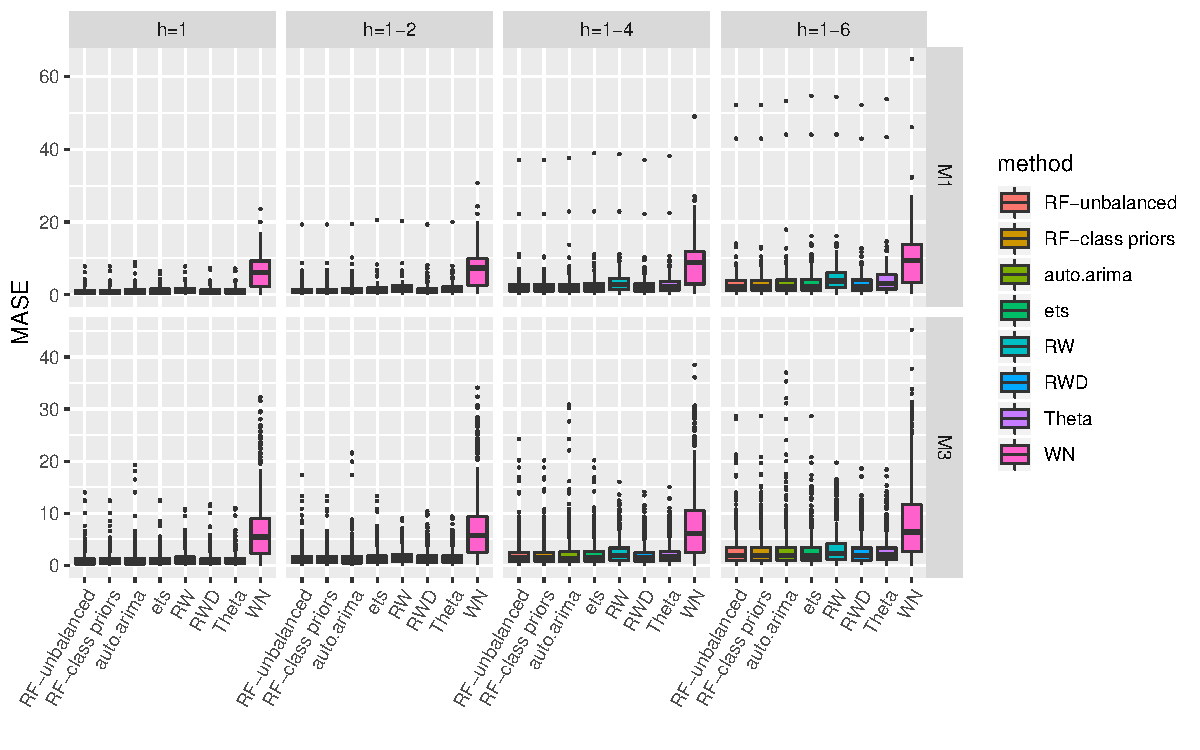
\includegraphics[width=\textwidth]{figure/yearlybox-1} 

}

\caption{Distribution of MASE values calculated over the new series for yearly data}\label{fig:yearlybox}
\end{figure}

\begin{figure}[H]

{\centering 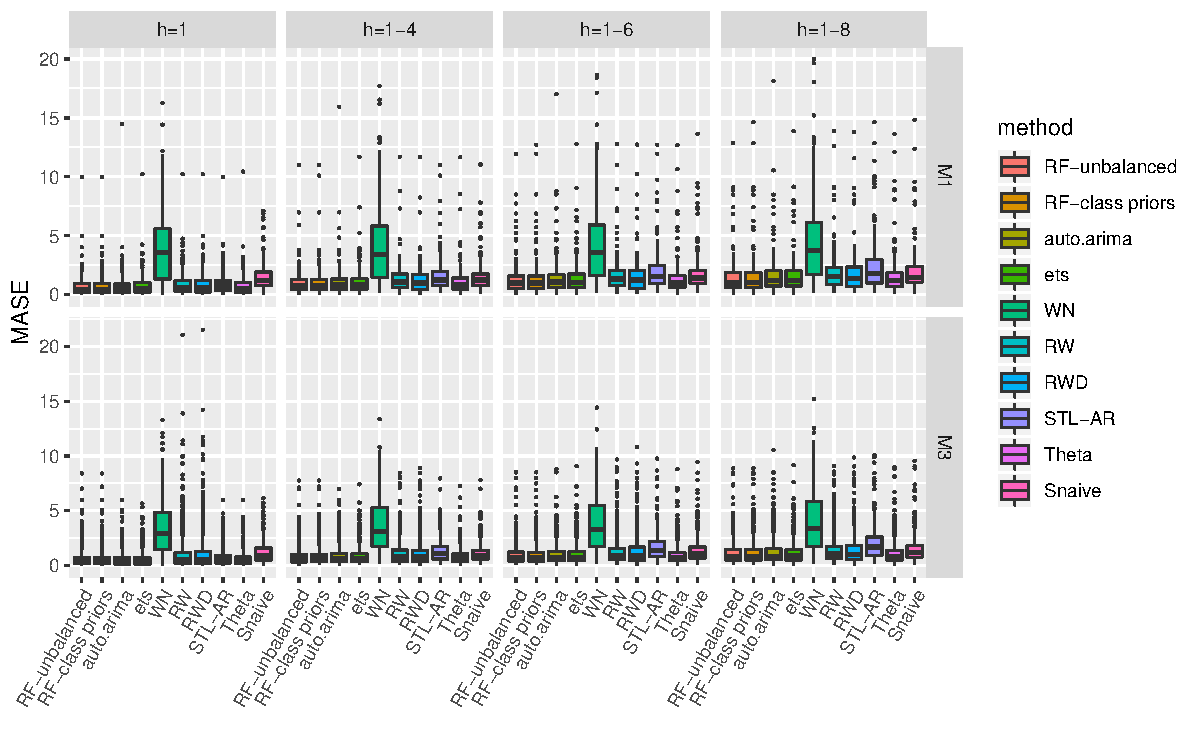
\includegraphics[width=\textwidth]{figure/quarterlybox-1} 

}

\caption{Distribution of MASE values calculated over the new series for quarterly data}\label{fig:quarterlybox}
\end{figure}

\begin{figure}[H]

{\centering 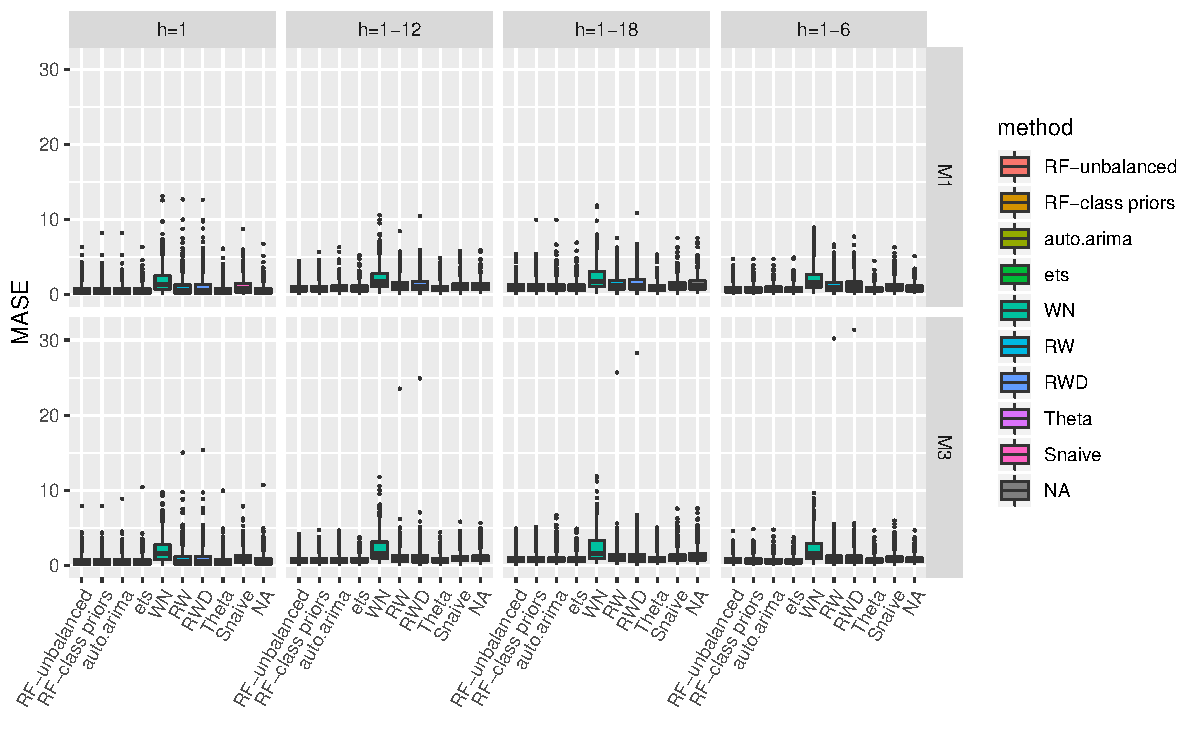
\includegraphics[width=\textwidth]{figure/monthlybox-1} 

}

\caption{Distribution of MASE values calculated over the new series for monthly data}\label{fig:monthlybox}
\end{figure}

\printbibliography

\end{document}
